\chapter{Language evolution}
\label{c:evolution}

The previous chapters have shown that huge advances have been made in the decade after the original Talking Heads experiment. 
It is now realistic to do experiments with physical humanoid robots, which was unthinkable 
in the late nineties. Whereas categorisation using 
basic perceptually grounded categories was a big achievement at the end of the nineties, experiments now routinely use 
complex compositional semantics. Another big boost has come from the development of a grammar formalism
(Fluid Construction Grammar) that is adequate from the viewpoint of linguistic complexity and allows at the same time
sophisticated experiments in grammar emergence. We now have several in-depth studies of language strategies for several 
domains although much more work obviously needs to be done to map out the vast landscape of language strategies found in 
human languages. This work is difficult and time consuming because each semantic domain generates its own set of fundamental 
problems in perception and action, conceptual representation, grammar, and language game interaction. 

But the sceptical observer will argue that most of these experiments are about language emergence rather than 
language evolution per se. Agents are given a certain set of strategies, which thus constitutes their 
innate Language Acquisition Device, and it is then demonstrated by computer simulations or 
robotic experiments (i) how these strategies are effective to {\itshape acquire} an existing language system in a 
population, (ii) how they are effective to {\itshape extend} a language system so that it remains adaptive 
to the needs and environments of its user, and (iii) how a population can {\itshape invent and coordinate} a new language system from 
scratch by using the strategy. 

Although long-term change is possible
given a particular language strategy (for example, new colour categories and colour terms might emerge
when needed to cope with new situations in the environment), this change does not alter
the set of language strategies available to the agent. Therefore - the critical observer would say - all this does still
not address the question yet where the strategies come from. 

\section{Culture-driven language evolution}

To clarify these issues, let us first define a distinction between emergence, language change, and evolution:\is{culture-driven language
evolution}
\begin{itemize}
\item {\itshape Language emergence} is the phenomenon whereby a language system, i.e. a set of conventions and conceptualisations
for a particular semantic domain, for example tense-aspect, colour, space or determination, arises in a population and 
becomes shared, based on a particular strategy (or a set of strategies) that is shared by all agents. 
\item {\itshape Language change} happens when the components of a language system and its conceptualisations shift, but the 
change remains within the bounds of a particular strategy. For example, the boundaries how different cases are used 
may shift (as is happening with the dative and genitive at the moment in German) or a new basic colour category and
colour word may arise and claim a region within the colour space (as happened with the word `orange' which 
started to be used as a basic colour word in 16th century Middle English to occupy a distinctive region between yellow and red). 
\item {\itshape Language evolution} occurs when new strategies arise. There is plenty of evidence from creole languages and 
from historical linguistics that this happens at a cultural time scale. Here are three examples:
\begin{enumerate}
\item Phrase structure (in the sense of 
strict word order based on abstract hierarchical patterns) emerged gradually in 
proto-Indo European, from a stage with largely free word order but a strong inflectional system \citep{VandeVelde:2011}. 
\item Word order and prepositions became the dominant strategy instead of morphological cases 
for expressing argument structure in the late Old English period \citep{VanKemenade:1987}. 
\item There is currently an evolution going on in Spanish clitics (`le', `la', `lo') whereby the etymological system 
of Standard Spanish, which uses clitics to express different cases (nominative, dative, accusative), is shifting 
to a referential system (expressing gender and number). Case differentiation is lost, but existing forms are recruited
for the new functions implied by a referential strategy  \citep{Fernandez-Ordonez:1999}. 
\end{enumerate}
\end{itemize}
It is not always obvious from the observation of language facts whether we are dealing with change (within the boundaries 
of a strategy) or with a new strategy. However, this becomes entirely clear when we try to computationally model the processes of 
acquisition, expansion or invention of the language strategy involved. We always try to understand change first using existing 
strategies until we are forced to introduce a new strategy because the differences at the conceptual or linguistic 
level are too profound to computationally handle them. 

The distinctions made here map to similar ones in biology. Biological strategies encoded in the genome govern the 
construction of phenotypes which include the form of organisms and their behaviours 
ensuring survival issues such as predator avoidance, food gathering, navigation, mate finding, nest building, etc. 
When we see a swarm of birds in the sky, or a path formed by ants, or a beaver dam, we see an example of 
{\itshape emergence}: A large-scale macroscopic structure emerges from the individual activities of the agents (i.e. animals)
without central control, similar to the way a language system emerges as a macroscopic shared structure
through the individual activities of the linguistic agents. The activities of the ants or the beavers are all governed by the 
same innate strategy. For example, to achieve path formation, ants put down pheromone when returning from the nest
and they follow pheromone gradients to find a path. 

Living organisms are {\itshape adaptive} to their environment and so even within 
the bounds of a given set of innate strategies there may still be significant changes observed in appearance, 
behaviour or internal functioning. For example, beavers 
may start using rocks for dams when mud and branches are not available, birds use plastics or other waste products, 
a goat may start to walk on two hind legs when it did not grow the forelegs \citep{Jablonka:2013}. 
Nevertheless true {\itshape evolution} is only said to happen if there are new innate 
strategies, i.e. genetically coded strategies, that arise, for example if a fish species genetically 
speciates into subspecies where one continues to bread eggs deposited on the bottom of the sea whereas the 
new variant does mouthbrooding, meaning that eggs are bred within the mouth of a parent. 
Also in biology it is not always clear whether we are dealing with adaptive change (without genomic change) or evolution
(with genomic change). Some variants that were thought to be a different species at one point of time
turned out to be ecotypes of the same species, i.e. variants that 
have the same genetics but a different appearance or behaviour due to adaptation to the environment. However today these debates
can be entirely settled when a genetic analysis is performed. 

For biological organisms, the standard approach to find out how (innate) strategies evolved is through the framework  
of genetic evolution by natural selection and it is logically possible that language strategies are also innate, in which 
case we should be able to figure out how they are genetically coded and evolved. 
There are indeed several researchers who strongly favour this hypothesis and they group their work 
under the banner of biolinguistics \citep{Boeckx:2013}. 

But it is also possible that language strategies are the outcome of cognitive development and cultural evolution, 
just like humans have developed a multitude of non-innate strategies in a wide range of domains: strategies for finding your 
way in cities, for building shelters, for preparing food, for playing Jazz piano, for fixing technical equipment, 
for organising trade, composing music, negotiating a contract, finding a partner, etc.  
This is the idea behind the {\itshape recruitment theory} of language evolution, which postulates that cognition and 
cultural evolution are the primary motors for the origins and propagation of new language strategies, even though of 
course they require the necessary neurobiological capacities that make each strategy possible. Once a strategy culturally 
evolved, it exerts a pull effect on genetic evolution, because genetic variants are favoured that can carry out a strategy more easily. 
So this hypothesis implies {\itshape culture-driven gene evolution} rather than gene-driven cultural 
evolution \citep{Fisher:2013}. 

It is this recruitment hypothesis \is{recruitment hypothesis}
that has been driving our experiments in language evolution and this chapter discusses very briefly
some of the experiments that explore this hypothesis with the same rigor and computational backing as 
the experiments in language emergence and change discussed in the previous chapters. Much remains to be done
before an experiment can be set up for evolving new strategies in some domain. 
We need to understand fully all the cognitive mechanisms 
required (both the semantic and the syntactic aspects). 
But since we now have at least a good technical basis and several concrete
case studies, as shown in the previous chapters, the study of language evolution, in the sense of the emergence and 
propagation of novel language strategies and their selectionist competition is within reach. 

What could a theory of cultural evolution look like? There is certainly no 
consensus on this.\footnote{See the debate in: \cite{Richerson:2005}.}
But the most obvious choice is to view cultural evolution as another instance of a Darwinian evolutionary dynamics, happening at 
the cultural and cognitive level rather than at the genetic level. This idea has been suggested by many researchers, 
including Richard Dawkins in his theory of memes \citep{Dawkins:1976}. 
The basic principle underlying Darwinian dynamics 
is to split the process of coming up with a design in three subprocesses: 
\begin{enumerate}
\item There is a process of {\itshape generating} possible variants, often by making changes to 
existing variants or by information transfer between variants, for example through cross-over. 
\item There is a separate process of {\itshape testing} whether these variants satisfy 
desired selection criteria. This happens usually in a kind of competition where different variants 
compete for available resources. 
\item There is a {\itshape self-enforcing causal loop} between the 
outcome of selection and the frequency with which a variant is maintained and hence used to generate new 
variants. 
\end{enumerate}
The last step makes Darwinian dynamics cumulative: Partly working solutions can be built upon further and lead 
the way to even better ones. 

Today, Darwinian evolutionary dynamics \is{Darwinian evolutionary dynamics}
is recognised as a general principle that can and has been applied to 
many different types of systems, in chemistry, neurobiology or 
economics.\footnote{See \cite{Arthur:1996}, \cite{Edelman:1987} and \cite{Luisi:2001}.}
It has also been used successfully to come up 
with new artificial systems, for example to evolve controllers for robots using 
genetic algorithms \citep{Nolfi:2000}. It is therefore not so surprising that 
selectionism can also be mapped to the cultural and more specifically to the linguistic domain in the following way: 
\begin{enumerate}
\item Speakers generate variants, either accidentally through errors in their speech production, or deliberately, 
for example, when they try to express a novel idea by inventing new forms or 
appropriating existing forms for new purposes, for example, by coercing a word or grammatical construction into a new usage. 
\item Which variants will survive in the communal language depends on selectionist criteria. I will 
discuss them shortly in more detail. They include for example whether the speaker is understood by the hearer, or whether 
it reduces the cognitive complexity of parsing and producing and hence allows larger sentences to be understood. 
\item The self-enforcing causal loop happens when variants created by one speaker start to propagate in the population 
and begin to replace their competitors. For example, a particular word to express a given meaning gets out of fashion 
and is taken over by another one. Some of these developments are simply fashion trends, but the more profound ones, 
in particular the ones that involve grammar, are related to critical selectionist criteria. 
\end{enumerate}
This Darwinian dynamic is already active in the operation of language strategies, since  a strategy regulates the 
creation and selection of variants, determines how feedback has to be handled, and implies a self-enforcing causal loop through 
lateral inhibition so that variants satisfying the selection criteria become 
dominant in the population. 

The key argument of this chapter is that the Darwinian evolutionary dynamics
also applies to the evolution of new strategies, which implies that (i) speakers and 
hearers have to be able to come up with new language strategies, (ii) selection operates not only on the level of choices given 
a strategy, but also at the level of the strategies themselves, and (iii) there is competition between strategies 
and a self-enforcing causal loop based on the success that language users have with the language system they created 
with a particular strategy, so that some strategies survive and become dominant and others fade away. 

Linguists are often reticent to use a selectionist approach because they believe that language is 
maladapted \citep{Boeckx:2005}. However we have to keep in mind that: (i) An evolutionary process 
seldom comes up with the perfect solution, even though it is remarkable effective given that there is no 
enlightened intelligent designer. (ii) There are conflicting criteria so that there is no optimal solution. 
For example, the speaker may want to minimise the effort needed for producing and pronouncing a sentence but this 
may make it harder for the hearer to reconstruct an interpretation of the meaning. (iii) Some of the selectionist 
criteria have to do with processing. A linguistic theory that only focuses on competence has nothing to say about 
processing and therefore cannot lay bare how processing issues play a role in language evolution. (iv) It is often possible 
to maintain communicative success with a simpler system (even a purely lexical language without any grammar at all) and then 
gradually optimise semantic interpretation by the progressive introduction of more grammar - as we see indeed 
in the emergence of creole languages which regenerate syntactic complexity from 
a lexical language \citep{Mufwene:2001}. 

What kind of selectionist forces are relevant in the case of language? \is{selectionist forces}
Clearly, the bottom line is that language users want to achieve {\bfshape communicative success}. 
Communicative success means that the speaker achieves his or her non-linguistic goal. For example, if a speaker
wants a hearer to perform some action (such as `Can you get me the car keys?'), there is communicative success if 
the hearer indeed performs the requested action. Speakers and hearers generally do not care whether their sentences
are perfectly grammatical or complete or semantically accurate. Speakers assume that hearers are intelligent enough
to infer the missing information and that they can fill in the required details from the context. 
In normal spoken dialogue, communicative success is immediately obvious, either 
from the actions that the hearer performs as a consequence of an utterance or by gestural cues whereby 
the hearer informs the speaker that he or she is being understood. 

Communicative success rests on a number of features of a language which thus act as key 
selection criteria: 

\begin{itemize}
\item {\itshape Expressive adequacy}: The language systems available to the speaker and the hearer must have 
the necessary expressive adequacy to reach communicative success. 
The available conceptual systems must include the needed conceptual distinctions 
and the available linguistic systems must be able to express these distinctions. Expressive adequacy depends 
not only on the goals of the speaker and the available embodiment but also on the environment. For example, 
if only black-and-white pictures are available, a strategy based on hue is entirely inadequate. On the other hand, 
if one of the dialogue partners is colour blind, a hue-based strategy would not work for coloured pictures. 
\is{expressive adequacy}

\item {\itshape Cognitive effort}: In order to cope with the incredible speed of normal language production and comprehension, 
reducing cognitive effort is of primordial importance. Cognitive effort is expended at all levels
of language: How much time and memory 
needs to be spent in coming up with adequate conceptualisations? How complex is the process of constructing
a sentence? How 
difficult is it to articulate the speech sounds? How efficiently can the sentence be parsed? How complicated is the 
interpretation of the sentence? If sentences are too 
complex to comprehend, for example because they trigger a large amount of combinatorial search, then 
hearers give up. Or if sentences 
are too hard to produce, the production process will be too slow to maintain the hearer's attention. 
Optimisations of cognitive effort are often in conflict for speaker and hearer. What requires less effort for the 
speaker might mean more effort for the hearer and vice versa. 
\is{cognitive effort}

\item {\itshape Learnability}: Speakers must occasionally expand their language systems to express novel meanings or 
better capture the attention of hearers with a ``fresh'' way of saying something. But these innovations will 
lead nowhere if they cannot be acquired by hearers. They will lead to communicative failure and 
the innovation will not propagate in the population and therefore it has no chance to survive in the shared language.
Learnability depends on whether speaker and hearer share the same language strategies, how much additional context 
is available, and how far the speaker has stretched established conventions to achieve his communicative goal. 
\is{learnability}

\item {\itshape Social conformity}: Speakers and hearers can greatly optimise their language production and 
comprehension by making their language systems as similar as possible. Moreover, details of language use, such 
as pronunciation, signal to which group a speaker belongs, and speakers often seek social conformity with the 
language use of their peers in order to belong to the group. Or they mimic the language systems 
of the most prestigious group in order to show they belong to that. The opposite happens as well. Speakers 
may try to mark themselves as linguistically different from a group to which they do not want to belong. 
\is{social conformity}
\end{itemize}

Language users certainly cannot consciously construct their language to satisfy 
these selectionist criteria, even if they would want to. They can have no 
foresight about all the possible distinctions that are going to be relevant in their world because new objects, 
new artefacts, new types of interactions always come up. They have no obvious way to know 
consciously how much cognitive effort a particular sentence is going to require from the hearer. They
cannot know in advance whether a metaphorical extension will be understood or whether the coercion of a 
word into a new grammatical function is going to be grasped by the hearer. And they cannot know for sure 
what the norm is in the group because they have no general overview, but can gain evidence only from 
local interactions with others whom they might not even be sure of whether they belong to the 
same group. The only thing they know for sure
(and not even always or immediately) is whether a communicative interaction was successful. 
This is why language evolution has to be a selectionist process. Language users are able to generate or reuse 
certain variants but they can never be absolutely sure whether these variants satisfy the linguistic selection 
criteria that would lead to more adapted persistent communicative success.

\section{Fitness landscapes}

Organisms use a variety of strategies for survival and offspring production:
bodily shape and appearance, specific sensors and actuators, metabolism, 
innate behaviours. Biologists call the ecological area that a particular organism occupies 
thanks to its physiological and behavioural strategies its ecological {\itshape niche}. A niche is defined through the ecological conditions
(temperature, altitude, habitat type, food availability, presence of predators, etc.) for which the organism's strategies
are appropriate and hence within which the species reaches a sufficiently high fitness to survive and fend off predators. 
Organisms may also have strategies to alter their environment so that some of their strategies become more possible or more optimal, 
a process called {\itshape niche construction} \citep{Odling-Smee:2003} \is{fitness landscape}

Niche analysis is performed by defining a multi-dimensional space, further called the {\itshape niche space}. Each 
dimension or {\itshape niche factor} has to be dealt with by the species in order to remain viable. There 
is consequently a direct
relation between the dimensions of the niche space and the selectionist pressures on the organisms trying to flourish 
within that niche which form a fitness landscape. Niche analysis
 typically examines how the different species within a delineated geological area 
are located within the niche space. It is then possible 
to see how species overlap, how they compete, how they are complementary, or whether some species are beginning
to occupy a niche left open by others. Usually the dimensions of the niche space are not known but have 
to be inferred through multi-variate analysis from empirical observations of species occurrence and 
detailed descriptions of environmental factors \citep{Elith:2009}.  But it is also possible to 
operate in a top-down manner, based on prior analysis of what might be niche factors, and to manipulate the environment 
to detect under what conditions the members of a species will thrive or not \citep{Nosil:2008}. 

By analogy with biology, we can apply the concept of a niche to the evolutionary study of
language systems and language strategies. To investigate linguistic niches in a systematic way, we need to identify first 
what factors are relevant. Some of these factors 
have to do with external conditions, for example, if the language games require expressing fine-grained hue distinctions or 
temporal and aspectual distinctions. Others relate to internal conditions, for example, how big is the search space during parsing, 
how much does a model of the situation need to be consulted. Next we can 
examine the performance of different systems and strategies for these factors, and map performance as 
points or regions in the niche space. Then we can study whether these points move towards greater or lesser optimality over time, 
how different systems or strategies compete when occupying the same niche, or how language systems and language 
strategies adapt to changes in the ecological conditions and hence the dimensions or critical values
of the niche space. The factors relevant for a linguistic niche include the selectionist criteria discussed earlier, 
and they can be analysed by identifying a fitness landscape, where each dimension is a selection component. 
I discuss first examples of this kind of analysis for language systems and then for language strategies.

\subsection{Fitness landscapes of language systems}
% {\bfshape Fitness landscapes of language systems}\\

To illustrate this approach let us look at a first example, \is{German article system}
using a fascinating study conducted by Remi van Trijp of change in the German article system as historically 
observed over the past 10 centuries.\footnote{
This section draws on the following publications: \cite{VanTrijp:2013} and \cite{VanTrijp:2013b}.}
The change is puzzling, because the article system started from a rather clean 
design in old High German to retain only a few forms in contemporary German. This contemporary system 
seems to be maladapted because the same forms are now used for many different purposes (syncretism) causing 
uncertainty and hence combinatorial search in parsing. For example, in Old High German there was a three-way gender 
distinction between masculine, neuter, and feminine for both nominative and accusative plurals, but in New 
High German only one form `die' is left. 
Many linguists have argued that these changes are just random, caused by phonological erosion and confusion 
of closely related word-forms. But van Trijp hypothesised that the changes 
were actually Optimisations, whereby speakers optimised their own cognitive effort at the cost of that of
hearers, even though the reduction in system complexity stopped 
at a critical point to preserve the disambiguation power of the system. See \figref{fig:german}. 

\begin{figure}[htb!]
\centerline{
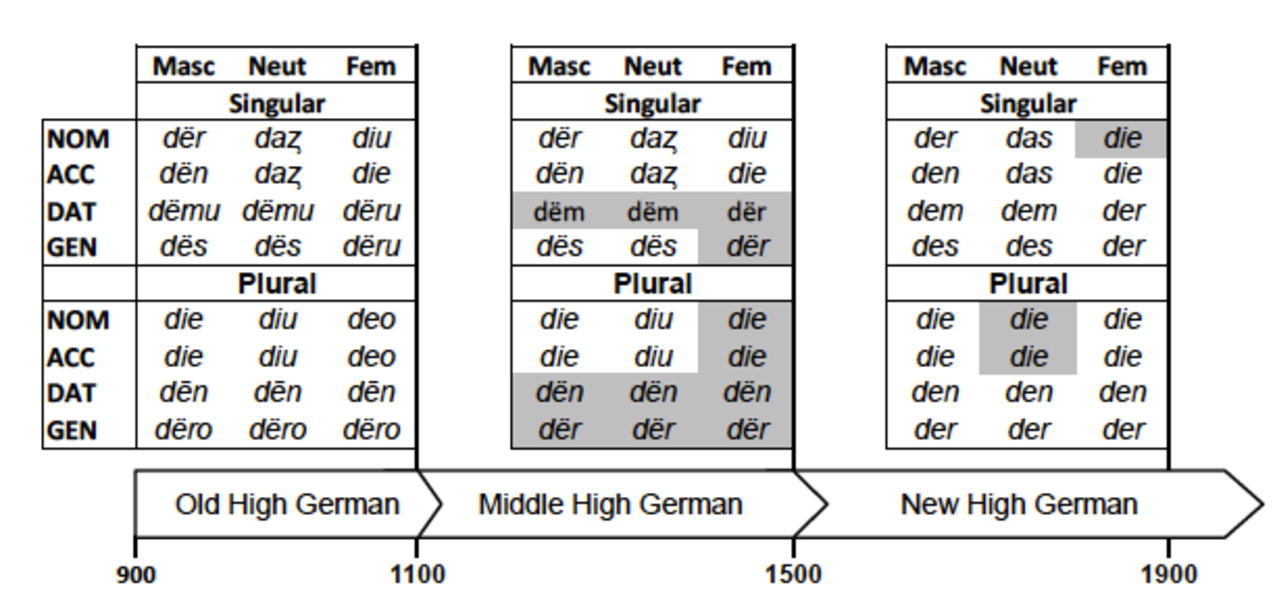
\includegraphics[width=0.75\textwidth]{chap12/figs/german-system.pdf}
}
\caption{{The German article system has morphological marking for case (nominative, accusative, dative, 
genitive), number (singular, plural) and gender (masculine, feminine, neuter). The system simplified 
from a well-structured clear system in old-high German to a system with more syncretism (the same form used
for multiple purposes.) }
\label{fig:german}
} 
\end{figure}

Van Trijp initialised three populations of agents: with the Old High German system, 
the Middle High German system, or the New High German System. He then defined the following four dimensions for the 
fitness landscape: \enlargethispage{1\baselineskip}
\begin{enumerate}
\item {\itshape Search effort} which is the amount of search that is needed, scaled between minimum (when there is one marker for every of 
the 18 possible configurations and so no search is needed) and maximum (when there are no markers at all).
\item {\itshape Disambiguation power} which is based on the number of possible interpretations left after application of the grammar. 
The disambiguation power is also scaled with maximum power for 12 markers and minimum for 0 markers (not counting the genitive). 
\item {\itshape Articulatory effort} which is calculated in terms of the number of movements that articulators such as the lips and 
tongue have to make when pronouncing the different phonemes that make up each article. 
\item {\itshape Acoustic precision} which is based on the phonological distance between words.
\end{enumerate}
Criteria (1), (2) and (4) pertain to the hearer and (1) and (3) to the speaker. They are calculated for each utterance
in a corpus and the weighted average gives a value for the performance of the language system for each of these dimensions. The global 
performance can be assessed by taking a (weighted) average of each of the values for all dimensions. 
As expected, Old High German scores the highest for disambiguation power and acoustic precision and the lowest for articulatory effort 
and processing effort, thus being an advantage for the hearer but not for the speaker (see \figref{fig:german-system}). 

On the other hand, the New High German system manages to become equally effective for disambiguation while requiring less search effort
and articulatory effort, if other complementary cues are made available to the hearer by additional grammatical 
strategies, namely grammatical agreement between the article and the noun within a noun phrase, so 
that features of the article can be deduced from the noun, and syntactic valence of the verb, because that suggests
which cases noun-phrases and hence their articles may have. 
This demonstrates that we should not always focus on a single strategy alone 
but have to take other relevant strategies into account. 
Moreover some forms, which are not very distinctive from an acoustic point of 
view (such as `der', `den' and `dem'), and therefore risk being collapsed into a single form, are 
nevertheless maintained because they are needed to resolve ambiguities that are not mitigated by 
other syntactic devices. This shows how an evolutionary point of view helps us to formulate explanatory hypotheses about language. 

\begin{figure}[htb!]
\centerline{
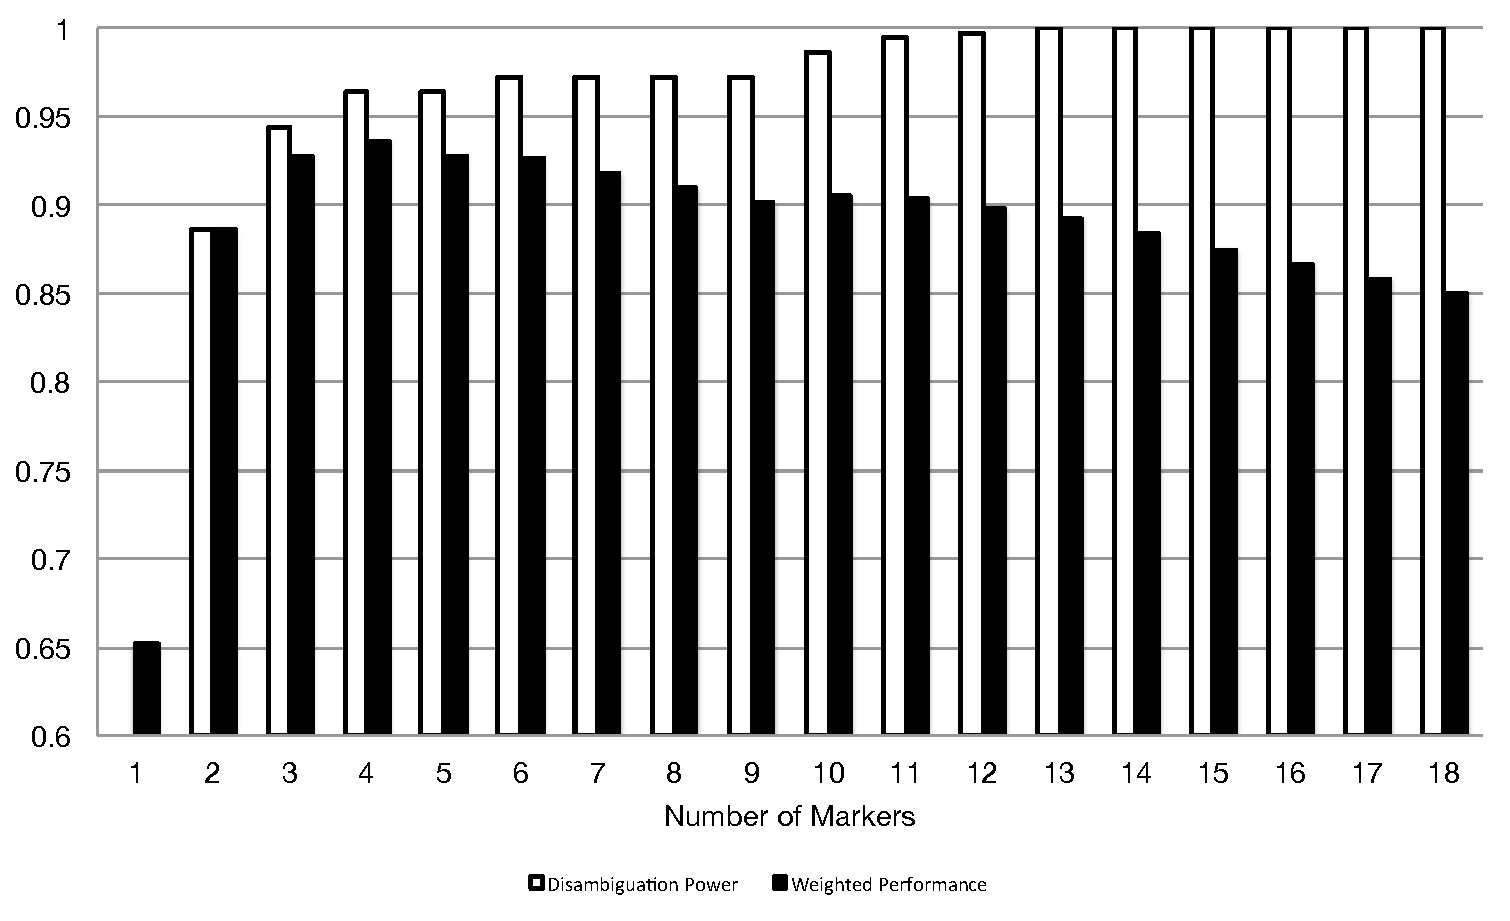
\includegraphics[width=0.75\textwidth]{chap12/figs/niche.pdf}
}
\caption{{Fitness landscape for the German marker system. When the number of markers increases (x-axis), the disambiguation 
power (y-axis) (which takes into account not only the markers themselves but also the other cues available for distinguishing 
gender and number) goes up. However the total performance for all four dimensions (y-axis) (which includes articulatory effort and 
search goes down). The optimal performance is reached for 4 markers (New High German has 5 markers whereas old High German had
9. \label{fig:german-system}}
} 
\end{figure} 

This example shows how it is possible to analyse the fitness landscape for stages of a language system at different points in 
time. The same analysis can also be done for different regional variants that are currently competing to become dominant 
in the standard language. An example of the latter is the currently ongoing evolution
from the etymological Spanish pronoun system to the referential pronoun systems, 
which has three different possible regional variants: `le\'ismo', `la\'ismo' and `lo\'ismo'. 
Van Trijp showed how each of these variants could equally arise with the same referential strategy and how it is 
a matter of historical contingency which one becomes dominant. Indeed we see that different regions of Spain
have chosen different variants \citep{VanTrijp:2010}. 

Here is another example of a fitness landscape from the domain of space, developed by 
Michael Spranger.\footnote{These results are documented at length in: \cite{Spranger:2014}.}
It focuses on understanding the role of grammar for optimising spatial language. \is{Spatial Language Game}
The experiment involves \textsc{qrio} humanoids
(see \figref{fig:spatial}) and uses a 
sophisticated vision system developed by Spranger, together with IRL and Fluid 
Construction Grammar (in the previous chapter).
\enlargethispage{1em}
A variety of spatial language strategies 
were operationalised, in particular: 


\begin{figure}[b]
\centerline{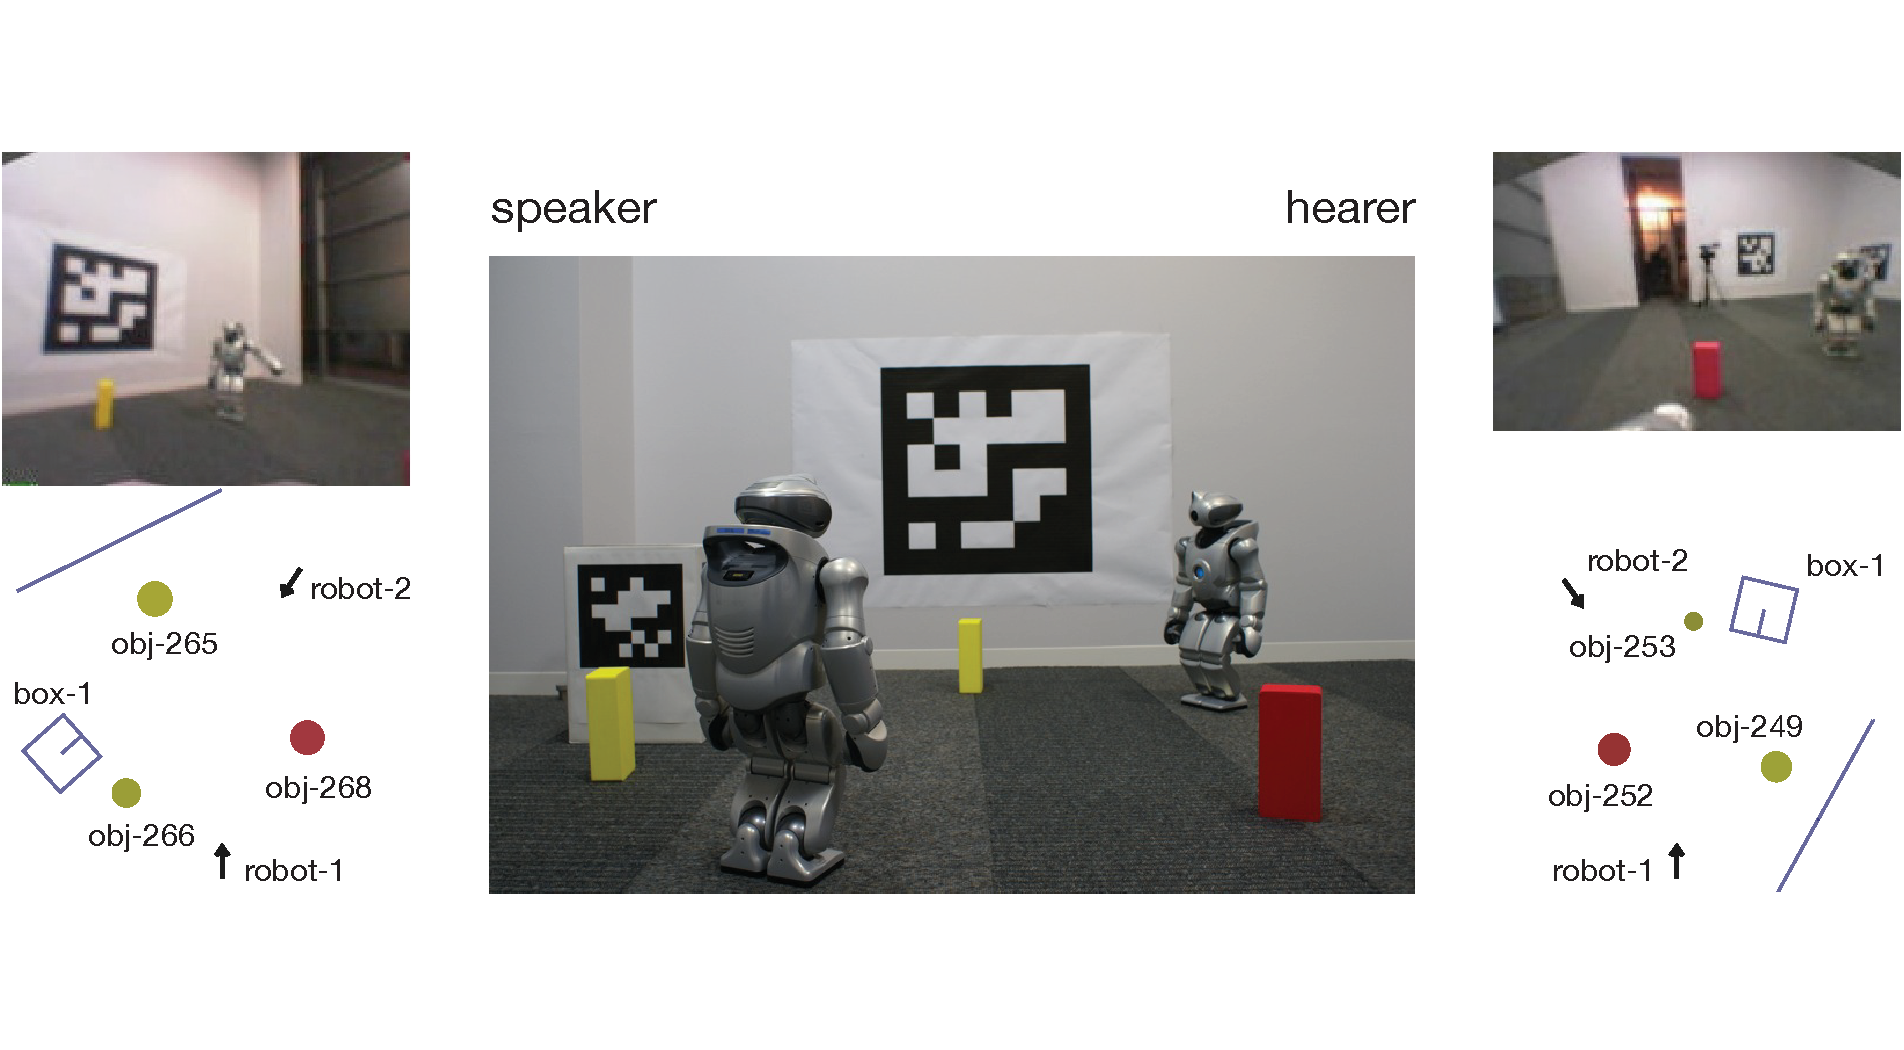
\includegraphics[width=0.8\linewidth]{chap11/figs/spatial.pdf}}
\caption{Set-up for the spatial language game experiments. Two robots are looking at a scene 
with a few blocks, a bigger box with tags indicating front, back or left and right side, and a global landmark in the form 
of a large tag pasted on the wall. {\itshape Top left and right:} World as seen through the camera of the robot. 
{\itshape Bottom left and right:} The internal world model as perceived by the left and right robot.}
\label{fig:spatial}
\end{figure}
\begin{enumerate}
\item The use of {\itshape projective relations} such as front/back, above/below, left/right. This requires imposing a coordinate
system on the world model and name areas within this coordinate system. A common coordinate system is to take 
an object, such as the human body of the speaker as reference point and project vectors emanating from the body. 
\item The use of {\itshape proximal relations} such as far/near. This requires that the distances of objects with respect to the 
reference point are computed and categorised. 
\item The use of {\itshape absolute relations}, such as North/West/East/South, related to global directions. 
\item The use of an {\itshape allocentric landmark} (as opposed to an egocentric one)
from which the situation is conceptualised. For example, in the 
phrase `the block in front of the box', the box is acting as a landmark and the projective spatial relations are 
computed as emanating from that object. Another example is `the block on your left' where the landmark is the 
hearer. 
\end{enumerate}

Spranger analysed the fitness landscape for grammatical strategies. He compared 
one population of agents that was initialised with a pidgin German, i.e. only a vocabulary for objects and spatial relations 
but no grammar, and another population initialised with a full locative grammar of German. He investigated three external 
factors: \clearpage
\begin{enumerate}
\item Scenes with many objects distributed around a landmark.
\item Scenes with several objects but no landmark that can be used as a spatial vantage point. 
\item Scenes with an allocentric and without an allocentric landmark but more complex with respect to number 
of objects and distribution of objects compared to (1). 
\end{enumerate}

\begin{figure}
\centerline{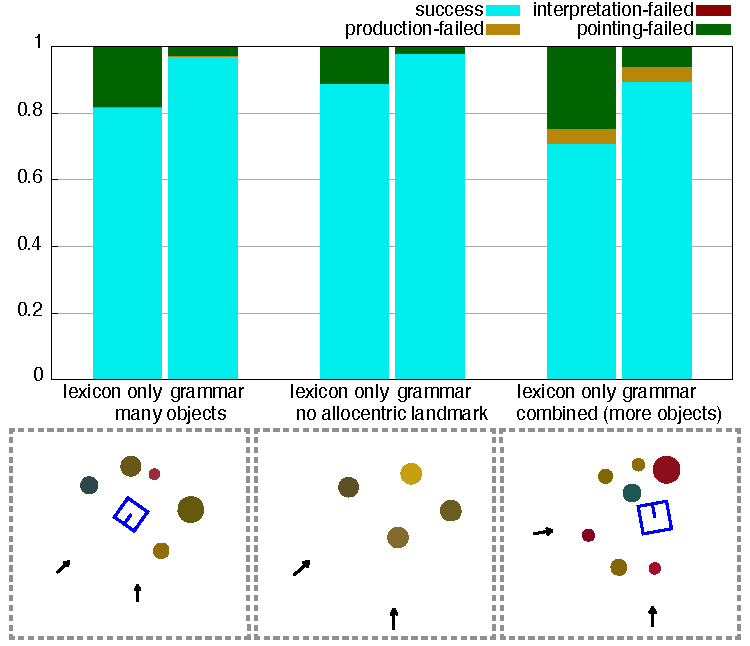
\includegraphics[width=0.5\linewidth]{chap12/figs/why-grammar-german.pdf}}
\caption{Investigation how the two language systems (lexical or grammatical) are performing with respect to the 
communicative success dimension and for each of the three ecological conditions. A purely lexical system in itself has 
already considerable success, but grammar becomes more and more relevant when the situation becomes more complex.
The bottom images show examples for the three ecological conditions being examined.}
\label{fig:why-grammar-german}
\end{figure}

Spranger used the following additional internal factors: 
\begin{enumerate}
\item {\itshape Communicative success}, including whether production failed, interpretation failed, or the hearer pointed to the wrong 
object (pragmatic failure). We see (\figref{fig:why-grammar-german}) that the more complex a situation becomes, the 
more grammar becomes relevant. 
\item {\itshape Semantic ambiguity}, being the number of semantic structures that remain after syntactic analysis and have to be mapped 
onto the perceived world in order to be disambiguated (See \figref{fig:ambiguity}, left). Without grammar there is a lot 
more semantic ambiguity and hence more cognitive effort to consult the world model. 
\item {\itshape Interpretation sharing}, which takes place when the semantic structure derived by the hearer is equal to that originally 
intended by the speaker (See \figref{fig:ambiguity}, right). Interpretation sharing is important in cases of displaced 
communication when agents do not have access to a shared world. We see that without grammar, interpretation sharing is 
heavily compromised. 
\end{enumerate}


\begin{figure}
\centerline{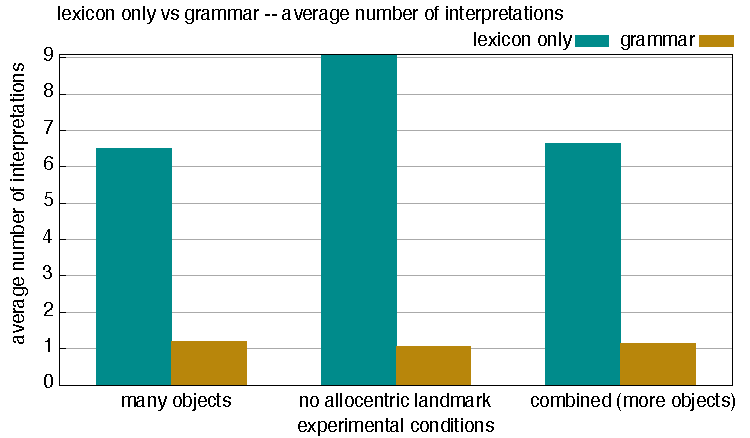
\includegraphics[width=0.5\linewidth]{chap12/figs/why-grammar-german-avg-interpretations.pdf}
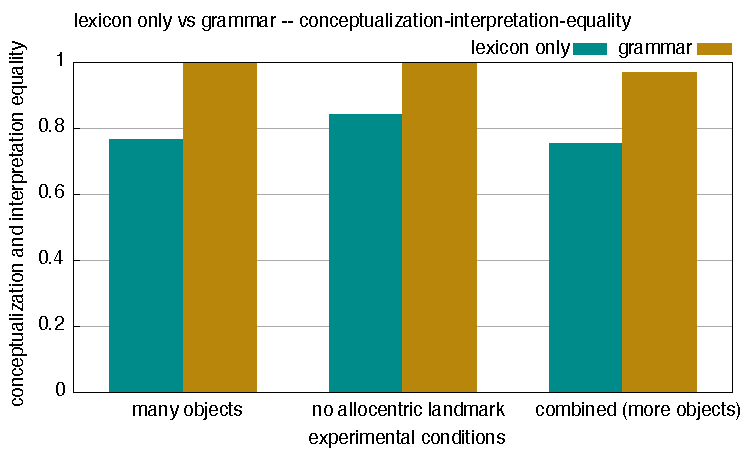
\includegraphics[width=0.5\linewidth]{chap12/figs/why-grammar-conceptualization-interpretation-equality.pdf}}
\caption{Left: performance for semantic ambiguity for the same three ecological conditions. We see that without grammar
the world model needs to be consulted heavily to weed out potential interpretations. And Right: Performance for interpretation sharing.
Only with grammar are agents able to share the same semantic structure, ensuring a higher degree of communicative success.}
\label{fig:ambiguity}
\end{figure}

\subsection{The fitness landscape of language strategies}
% {\bfshape The fitness landscape of language strategies}\\

We now move one level up, and show how a fitness landscape can be identified at the level of strategies as well. Rather than supplying 
agents with language systems, we initialise them 
with specific strategies, let them build language systems, and then examine the performance 
of these language systems for the different dimensions of the fitness landscape, so as to understand which niche 
the strategy occupies. Here is one example of this approach 
from the domain of color (developed by Joris Bleys).\footnote{These results are documented at length in: \cite{Bleys:2014}.}

The previous chapter already showed that there are 
different strategies for colour language: basic colour terms, graded membership (`very green'), compounds (`sky blue'), 
brightness qualification (`light green'), etc. All these strategies use a particular colour space, more specifically 
the CIE L*u*v* space where the L* dimension represents brightness (ranging from black to white), the u* 
dimension represents the red-green opponent channel, 
and the v* dimension the yellow-blue channel. This space was chosen 
because the distance between two colours in the L*u*v* space accurately represents 
the psychological distances between these colours as perceived by human subjects. \is{Color Description Game}

Let us focus on a family of strategies that all use a prototype-based approach, i.e. they perform categorisation using 
a standard nearest neighbour classification algorithm operating over an inventory of prototypical points, 
as also used in the Proper Naming Game and the Basic Colour Naming Game discussed in the previous chapter. 
Three variant strategies are imaginable (and can be found in human languages): \enlargethispage{2\baselineskip}
\begin{enumerate}
\item The {\itshape brightness-only strategy} which uses only the L* dimension (dark, grey, bright, etc.).
\item The {\itshape hue-only strategy} which uses only the hue dimension (blue, yellow, green, etc.). 
\item And the {\itshape full-colour strategy} which uses all dimensions. 
\end{enumerate}
In order to understand the niche of each strategy, Bleys has set up experiments where the context is controlled 
with respect to the importance of hue. 
For example, agents can be presented with contexts with samples where the hue is the same but brightness is different on the one 
hand versus contexts with samples where the brightness is the same but hue is different. In between we get a mixed 
importance of hue. 

\begin{figure}[htb!]
\centerline{
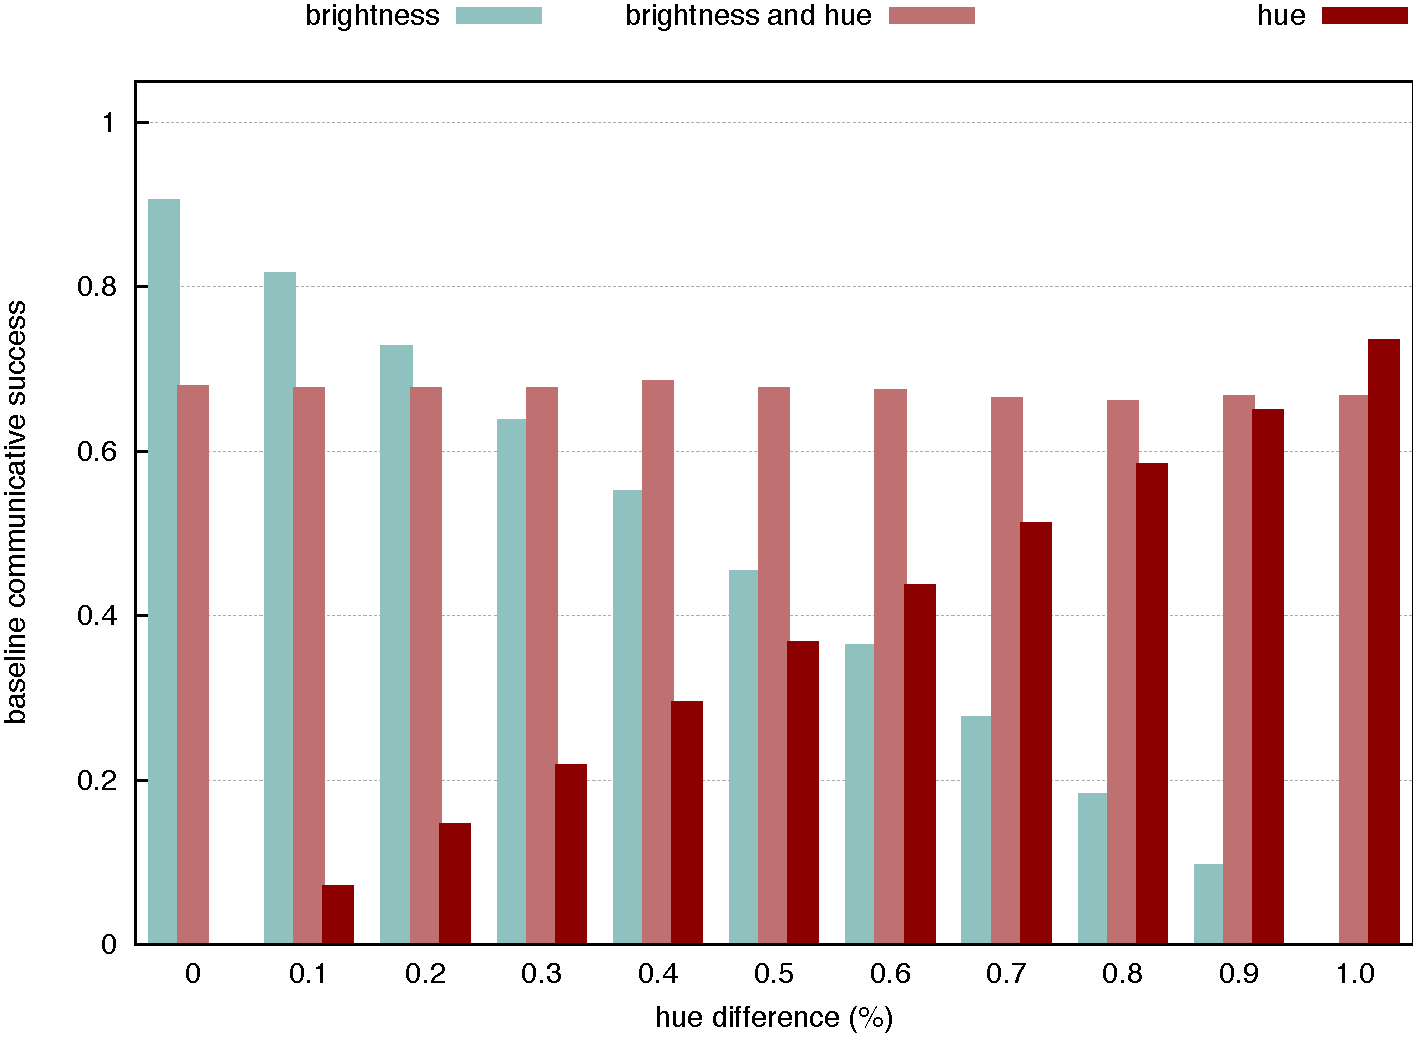
\includegraphics[width=0.6\textwidth]{chap12/figs/selective-advantage-bar.pdf}
}
\caption{{Niche analysis for three different 
colour strategies: brightness-only, brightness-hue, and hue-only. 
The properties of the context vary on the x-axis and the y-axis shows performance of each strategy.
Only one niche dimension is examined, namely communicative success. 
We see that each strategy has its own niche for which it is optimal, but the full-colour strategy is globally 
performing the best across contexts, which may explain why it has become preferred in most language families. 
\label{fig:bar}}
} 
\end{figure} 

Bleys initialised the three populations with the three different strategies and let them first learn an interpretation of 
the Spanish focal colours (with prototypes in brightness\-only, hue-only, and full-colour spaces). Then he measured 
performance for communicative success for the varying ecological conditions. 
Not unexpectedly, he found that depending on the percentage of the importance of hue differences in the context, a different strategy 
is more optimal (see \figref{fig:bar}). Not surprisingly, a hue-only strategy fails completely when the samples in each  
context have equal hue but different brightness, whereas a brightness-only strategy fails when the samples have 
equal brightness but different hue.

Another very useful type of experiment investigates in how far a particular strategy indeed makes a difference 
with respect to certain factors. Here is an example. It is again in the domain of spatial language discussed earlier and 
was conducted by Michael Spranger.

Recall that three internal factors were used 
for the fitness landscape in this domain: communicative success, semantic ambiguity and interpretation sharing. Spranger began with 
a population without any grammar but just a lexicon for expressing spatial relations and properties of objects. 
The agents were then initialised with a strategy that would build a grammar consisting of hierarchical
constructions which group all the components of a spatial relation, put them in a particular sequential order,
and add a marker to them. For example, a construction could arise that groups a spatial relation (like `front'), 
a determiner acting as selector (like `the'), and a noun introducing an object class (e.g. `box'), puts them 
in the order: spatial relation - determiner - noun, and adds a marker to them (e.g. `-bo'). 

\begin{figure}[htb!]
\centerline{
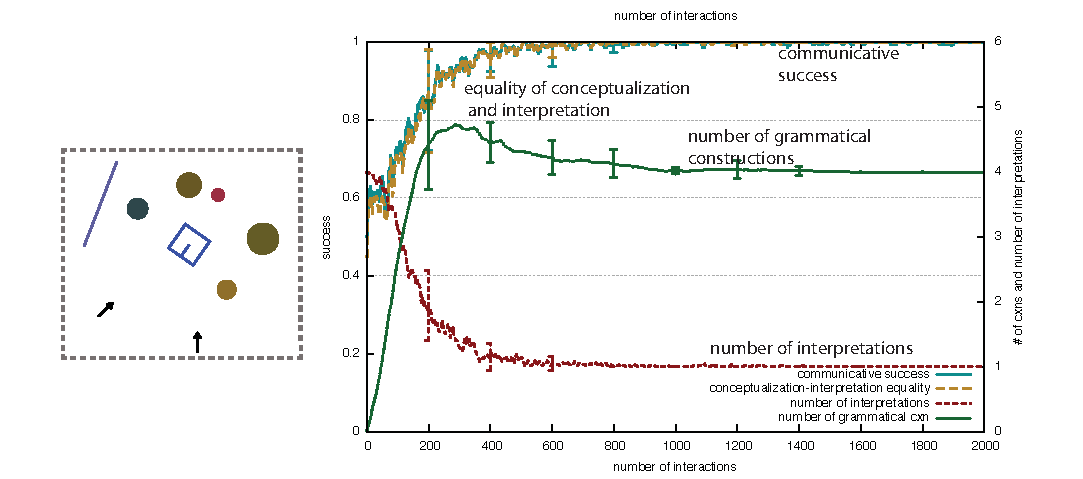
\includegraphics[width=0.9\textwidth]{chap12/figs/why-grammar-development-3.pdf}
}
\caption{{Agents have been given a grammatical strategy that introduces constructions to signal 
which conceptualisation strategy has been used and what its elements are. We see that communicative success and 
interpretation sharing go up to the maximum and semantic ambiguity (number of interpretations) goes down to 1, as 
the number of constructions built by the strategy increases. 
\label{fig:gramdev3}}
} 
\end{figure} 

A series of language games were played using contexts (such as the one shown in \figref{fig:gramdev3}, left)
that contained a wide range of objects and also a landmark stimulating the need for perspective reversal. As shown in 
the niche analysis earlier (see Figure \ref{fig:ambiguity} and \ref{fig:why-grammar-german}) a language without 
a grammatical expression supporting how spatial relations need to be analysed will reach a 
communicative success rate of only 70 \%. So the question is whether the agents will increase this success rate when 
they exercise this grammatical strategy. The same question can be posed for the other two niche factors (disambiguation 
and semantic sharing). Experimental results are shown in \figref{fig:gramdev3}. They confirm that as 
the language system is getting built up, key factors (communicative success, semantic sharing, and disambiguation) 
indeed get optimised, demonstrating that the strategy ``does its job''. 
\clearpage
\section{Selection and alignment of language strategies}

It is only one step now to achieve the selection and alignment of language strategies. Basically, two mechanisms needs to be 
added: \is{strategy selection}
\begin{enumerate}
\item Agents need to track the performance of their strategies by tracking the performance of the language 
systems that were built based on their strategies. In other words, not only lexical or grammatical constructions
but also strategies need to have a score. These {\itshape strategy scores} should be updated using the same 
lateral inhibition dynamics that we have been using at the level of word-meaning associations or 
more generally constructions. 
\item It is also necessary that the conceptualisations and the lexical and grammatical constructions that 
are implicated within a particular strategy are tagged with that strategy, so that if their score is updated, 
the score of the strategy can be updated as well (\figref{fig:tagging}). This is necessary  
for implementing a proper credit assignment 
mechanism and also for ensuring that a word becomes unambiguously used with a particular strategy. 
\end{enumerate}
The same word may be tagged with more than one strategy because 
a learning agent does not know which strategy has been used by the speaker and so this may lead to different
hypotheses. But in the end, agents strive for convergence so that they all use the 
same word with the same meaning. For example, a hearer cannot know whether a particular word (e.g. `yellow')
is to be interpreted using  the brightness-based or  the full-colour-based strategy, particularly
because both strategies could work in similar circumstances. For example, yellow colour chips are often the 
most bright ones and hence both strategies would work. Consequently it is unavoidable that different strategies compete
to recruit the same words, and this explains that we see this phenomenon indeed in the historically attested evolution 
of language. Indeed, many of today's hue words like `yellow', `brown' 
or `blue' were all expressing brightness-based distinctions in Old English before they became used as part of the  
Basic Colour Strategy in the late Middle English period (1350--1500).\footnote{See
\cite{MacLaury:1992} and \cite{Casson:1997}.}


\begin{figure}[htb!]
	\begin{center}
		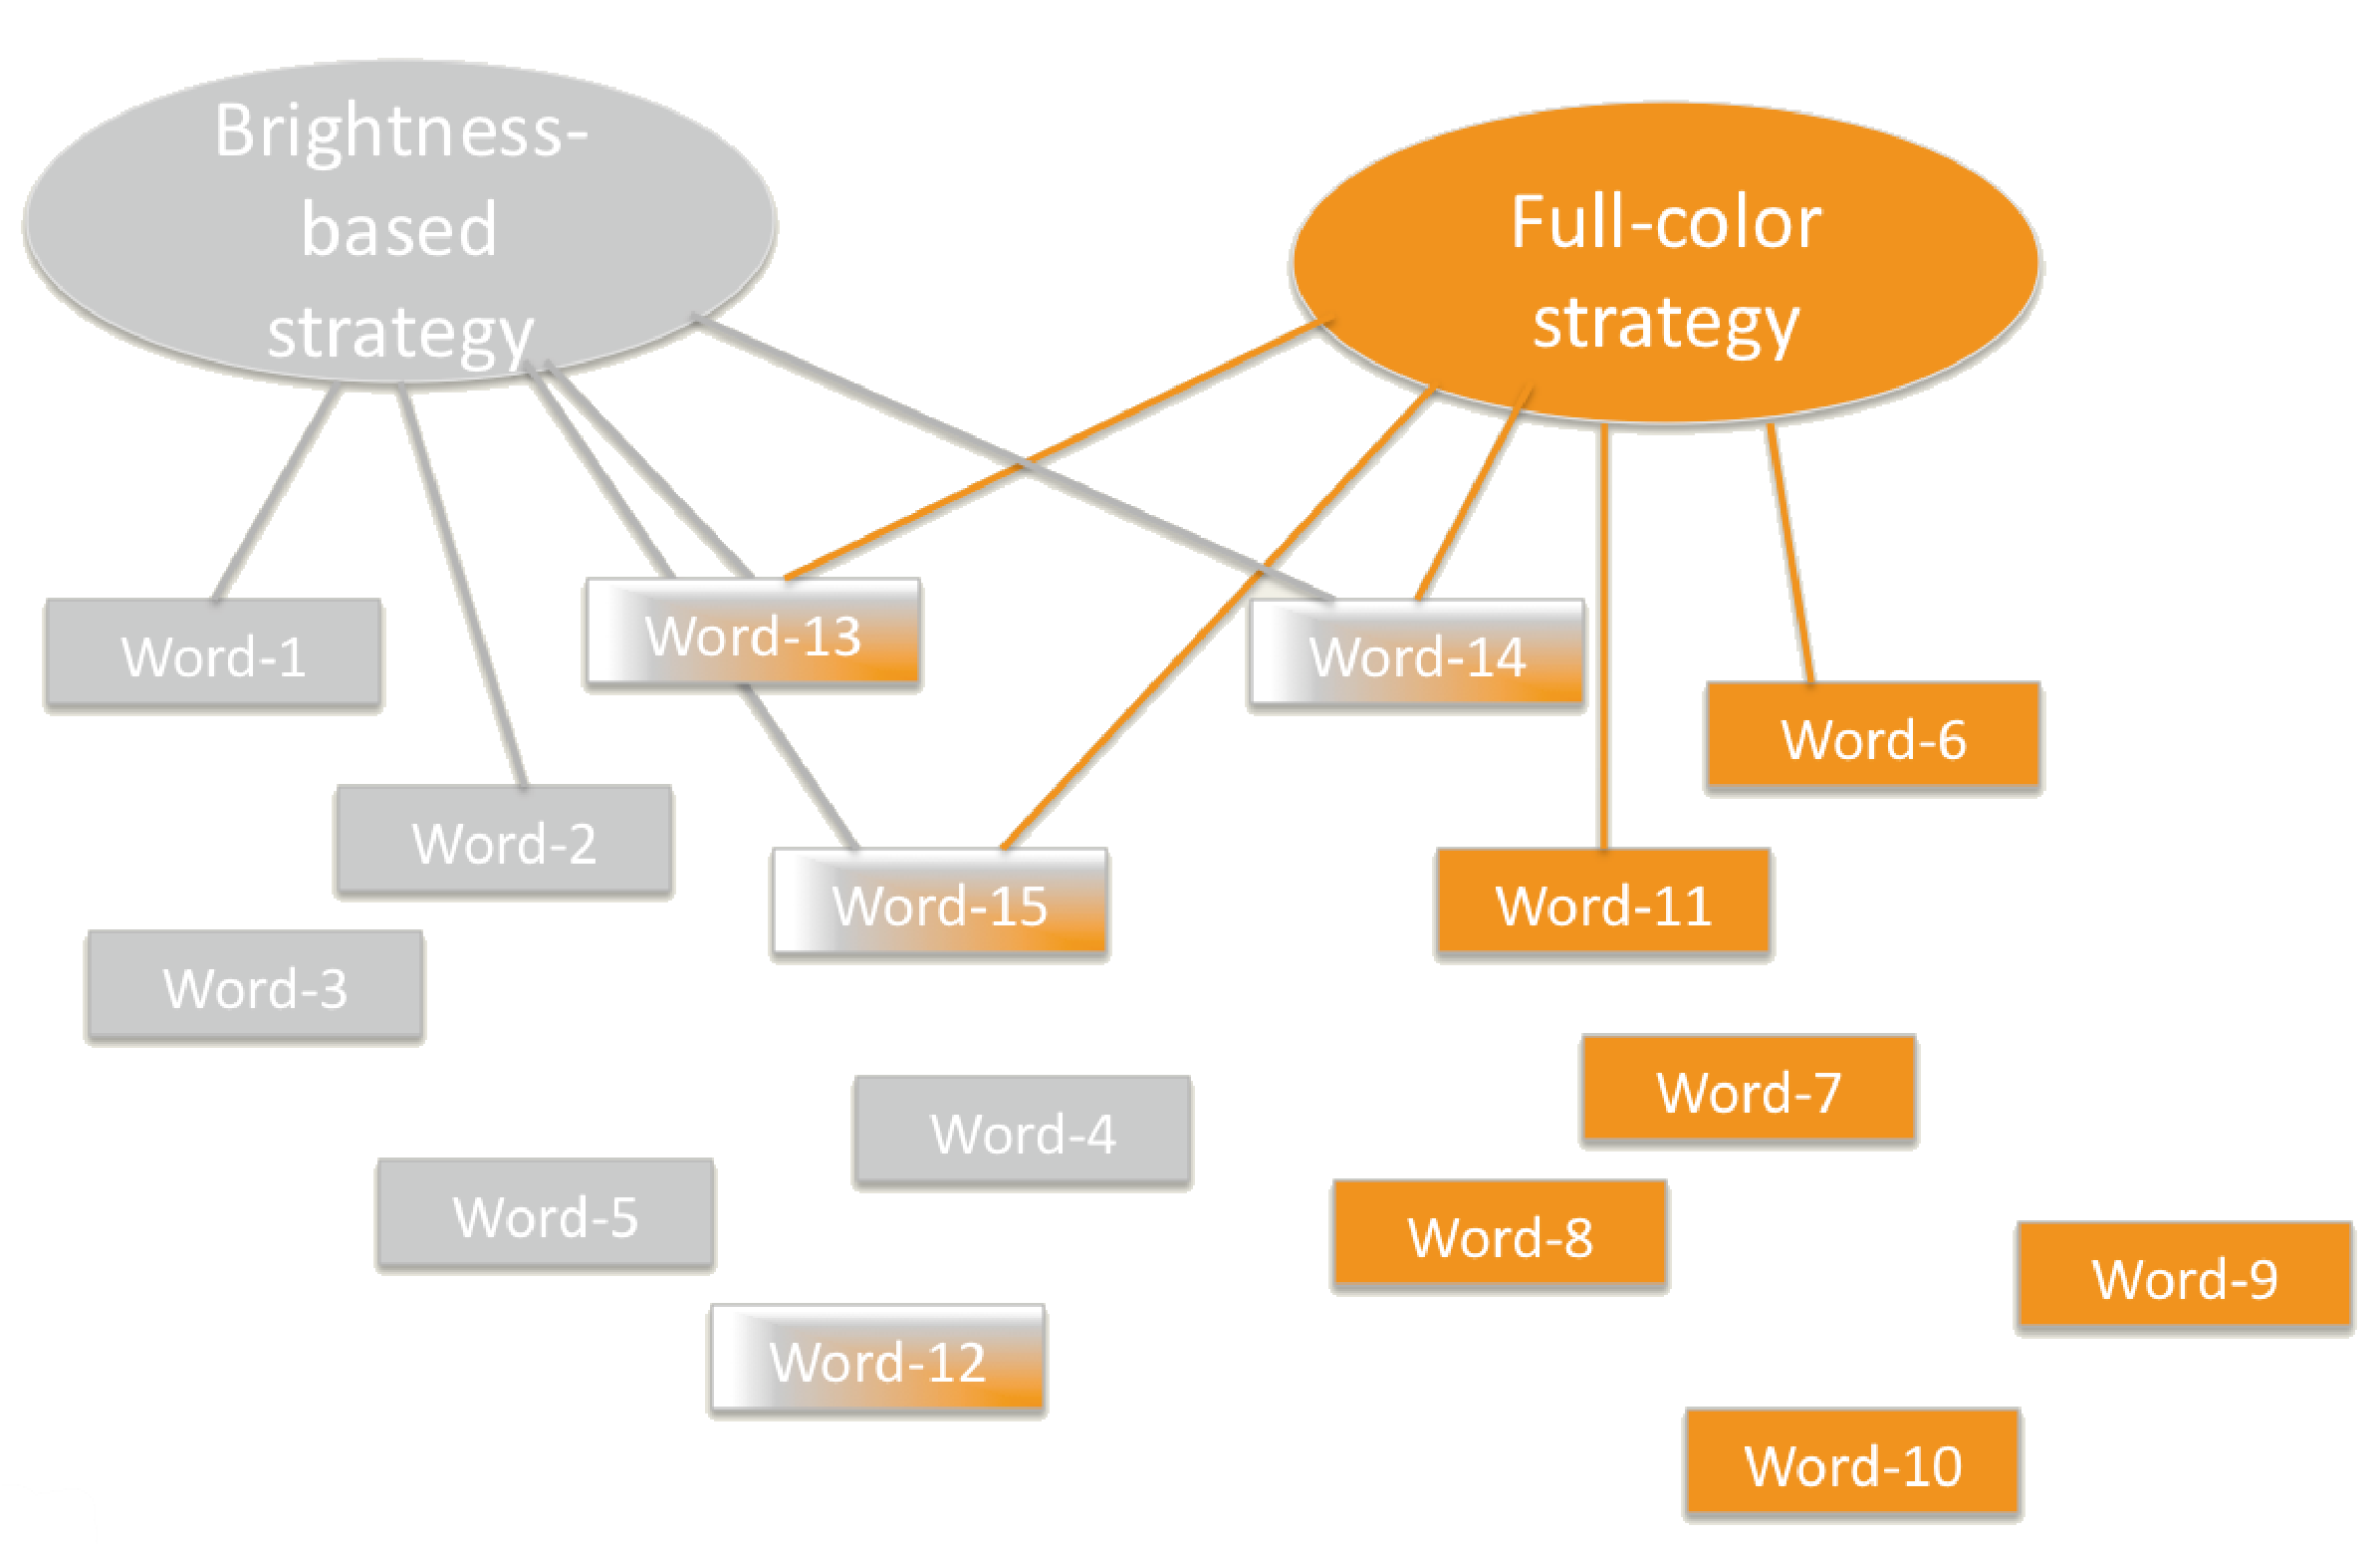
\includegraphics[width=0.70\textwidth]{chap12/figs/strats.pdf} \end{center}
		\caption{{Different words are tagged with the strategy with which they 
should be interpreted. This allows the operationalisation of a 2-level selectionist dynamics, operating at 
the level of strategies and at the level of the language system built with each strategy.
\label{fig:tagging}
}}
\end{figure}

We now look at an experiment, developed by Joris Bleys, which puts 
this evolutionary dynamics to work. This is very challenging because language users must reach 
agreement about a dominant strategy without central coordination and while keeping communicative success intact. 
The application domain is colour. 

The Bleys experiment concerns the brightness-based and the full-colour strategy. Both use 
a prototype-based nearest neighbour categorisation. We know from earlier experiments with the Proper Naming Game
and the Action Naming Game that this strategy enables a population of agents 
to self-organise a colour lexicon from scratch. \figref{fig:full-cs-dynamics} illustrates (on the left) how 
communicative success increases and the lexicon becomes more coherent, and (on the right) how the prototypes
of the different agents gradually expand and become similar to be almost identical after 1200 games per agent, when 
the system has stabilised to 6 basic colours. 


\begin{figure}[p]
\centerline{
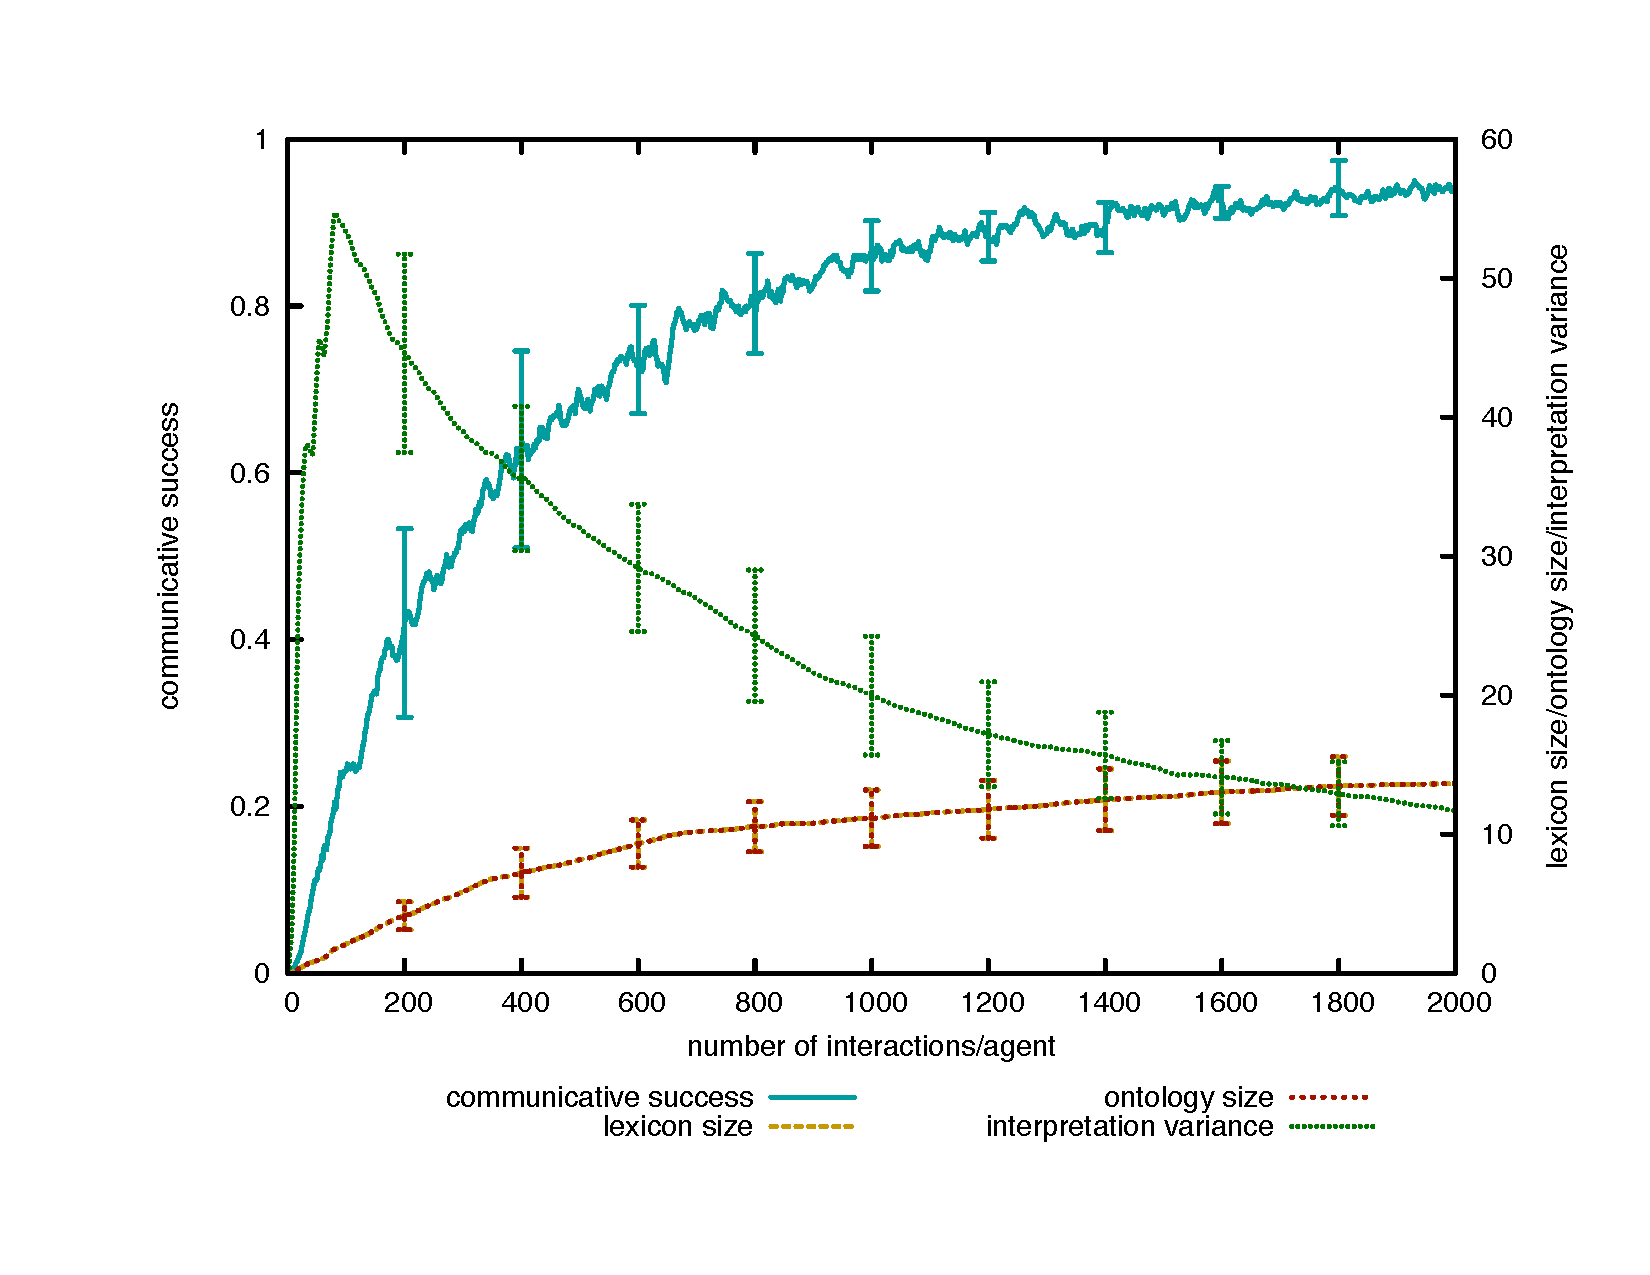
\includegraphics[width=\textwidth]{chap12/figs/full-cs-graph.pdf}
}
%\\

\centerline{
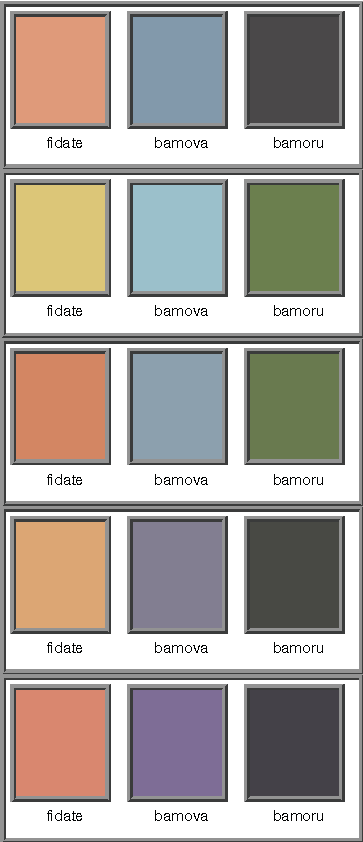
\includegraphics[height=0.5\textwidth]{chap12/figs/full-1000.pdf} ~~~
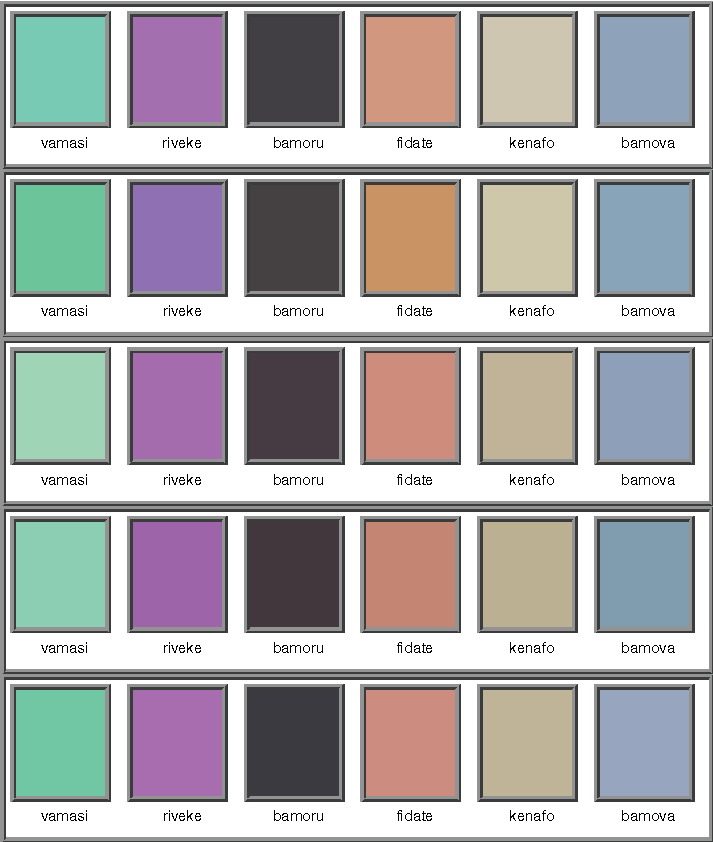
\includegraphics[height=0.5\textwidth]{chap12/figs/full-3000.pdf}
}
\caption{{The {\itshape Basic Colour Strategy} allows a population of agents (in this case 10) to self-organise a colour lexicon from scratch. The graph shows that high communicative success is reached with a lexicon of about 15 colour words (top). The evolution of a typical lexicon in a smaller population (5 agents), is shown after 400 (bottom left) and 1200 (bottom right) games per agent. Each row represents the lexicon of one agent.}
\label{fig:full-cs-dynamics}
} 
\end{figure}

The {\itshape Brightness Prototype Strategy} is similar to the Basic Colour Strategy, but instead of taking all three dimensions into account, only the L* dimension of both the stimuli in the context and the prototypes of the colour categories are compared. While learning, the prototype of the used colour category is shifted on the L* axis towards the L* value of the topic. During invention, only the L* value of the topic is considered relevant. \figref{fig:brightness-dynamics} shows that this strategy is also adequate to allow a population of agents to self-organise and coordinate a colour lexicon from scratch. The resulting colour lexicon now consists of different shades of grey. The set of prototypes also expands and becomes similar across agents. 

\begin{figure}[p]
\centerline{
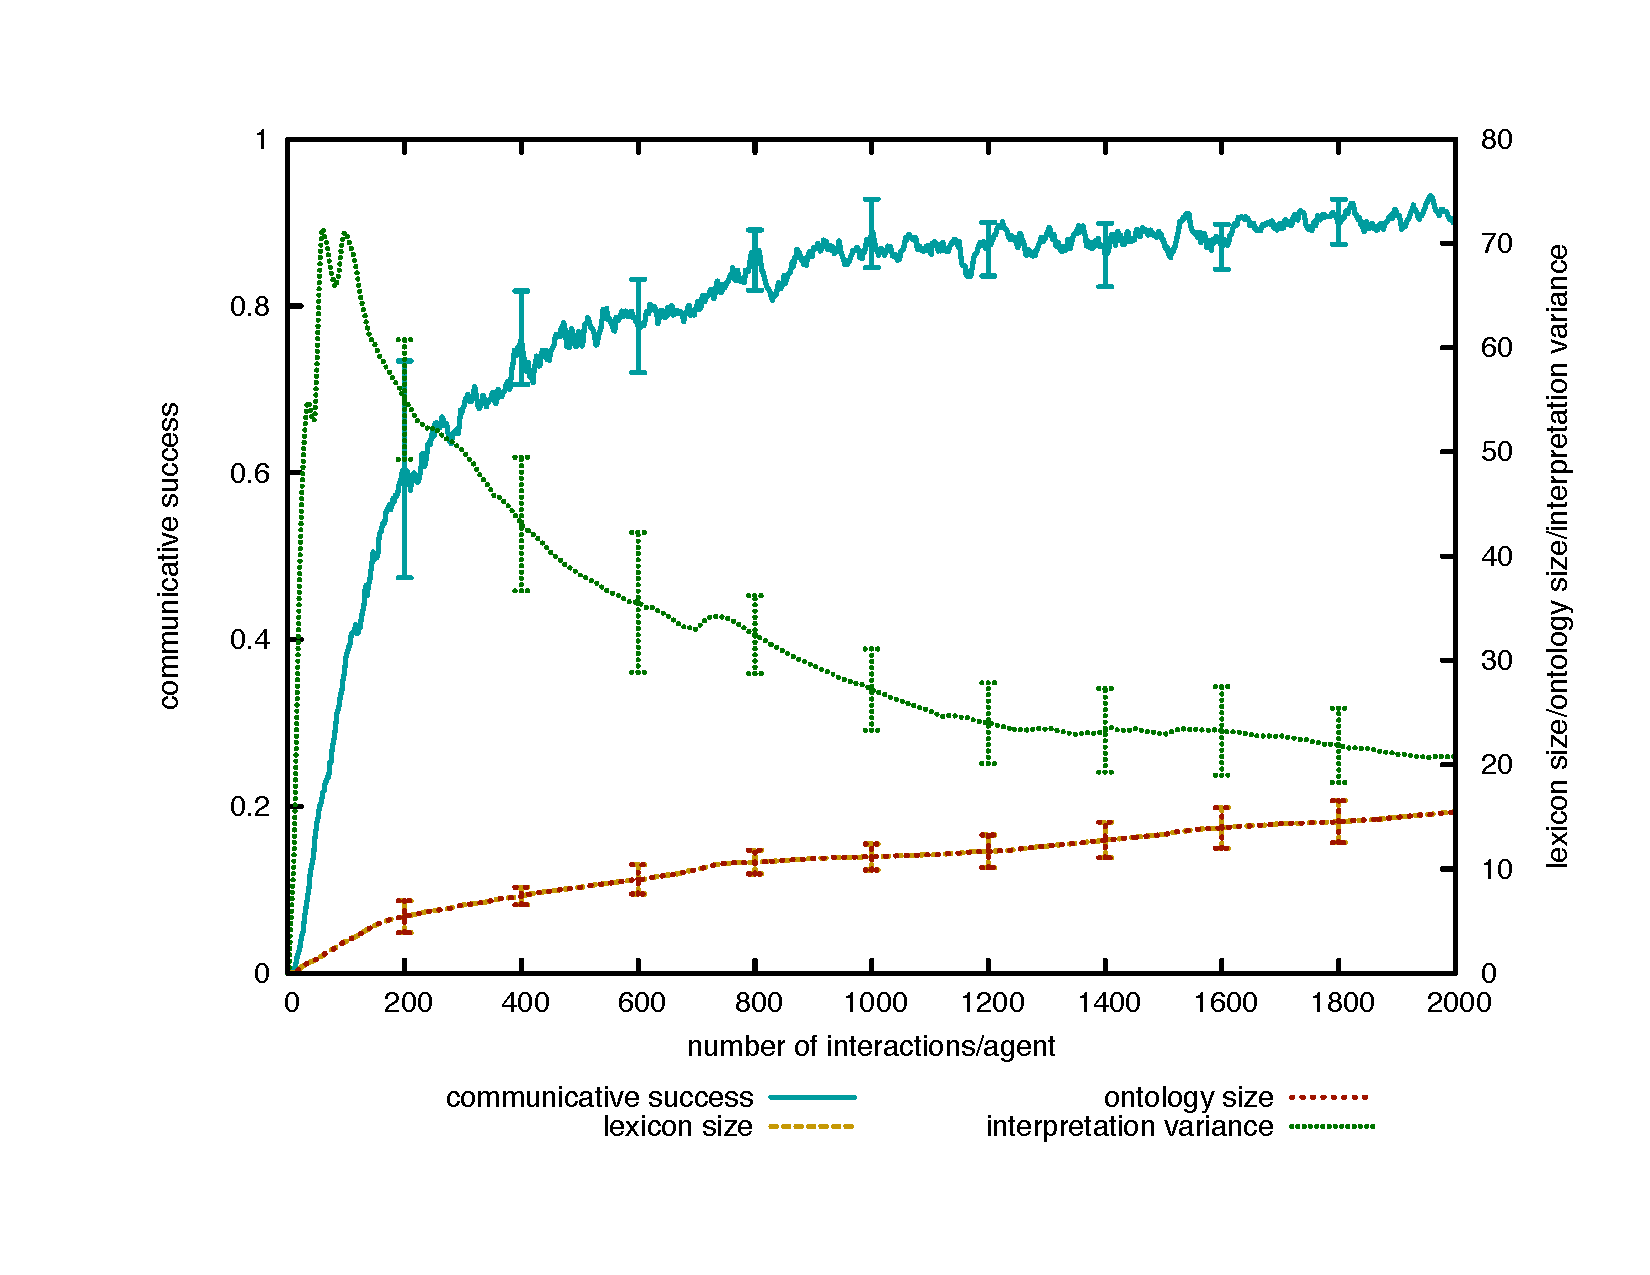
\includegraphics[width=\textwidth]{chap12/figs/brightness-graph.pdf}
}
% \\

\centerline{
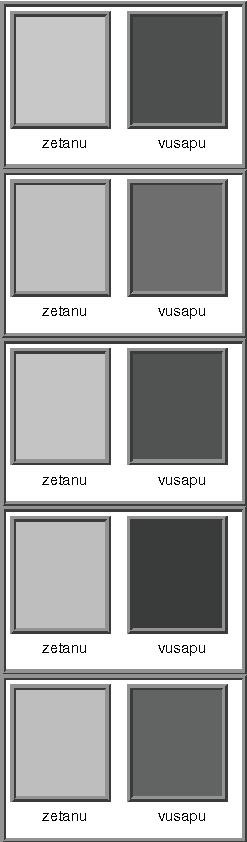
\includegraphics[height=0.5\textwidth]{chap12/figs/bw-1000.pdf} ~~~
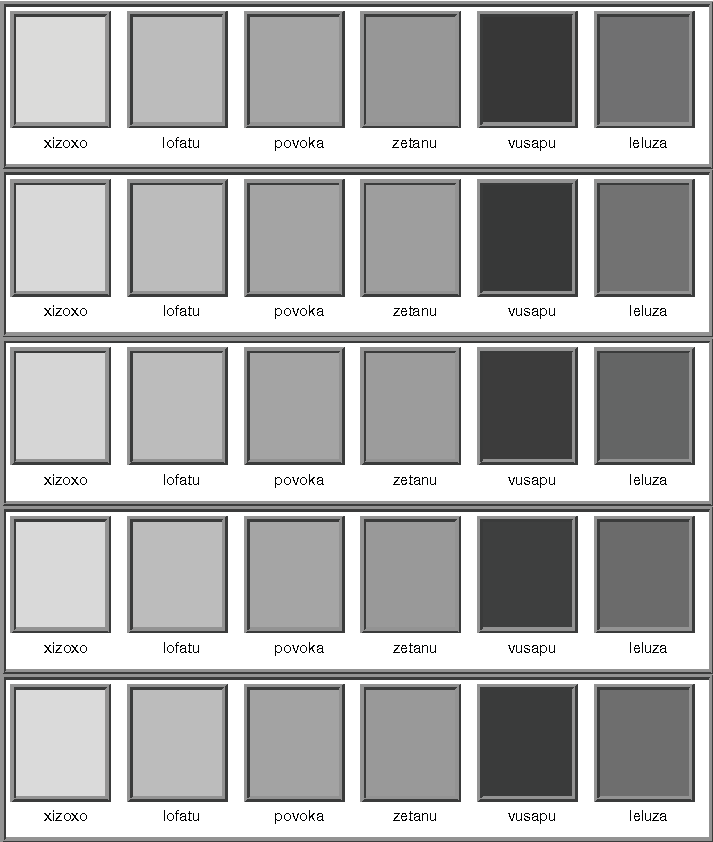
\includegraphics[height=0.5\textwidth]{chap12/figs/bw-4000.pdf}}
\label{fig:brightness-dynamics}
\caption{{The {\itshape Brightness Colour Strategy} also allows a population of agents (in this case 10)
to evolve an adequate colour lexicon (top). The evolution of a typical lexicon in a smaller population (5 agents), is shown 
after 400 (bottom left) and 1600 (bottom right) games per agent. Each row represents
the lexicon of one agent.}}
\end{figure}

We now turn to the main issue here: the
selectionist dynamics between both strategies. The following selectionist process has been implemented: 
\begin{itemize}
\item In speaking, agents handle a communicative problem with the solution 
that had most success in the past and this solution implies a particular strategy. 
When the problem cannot be handled, the speaker 
has to expand his set of meanings and his lexicon and he uses the default strategy, 
i.e. the strategy that had most success in the past, which translates into having the highest
strategy-score. It is only when this strategy does not work that 
other alternative strategies are tried out in decreasing order of their scores. 
\item In listening, the hearer first applies his own 
stored solution to interpret the utterance, which again implies the use of a language strategy associated
with this solution. When the hearer is confronted with an unknown word or with a situation in which 
his interpretation of the word does not work for the present context (because apparently the speaker 
used another strategy for this word), he uses first his own default 
strategy to figure out the meaning of the unknown word, and, if that does not work, he tries out alternative
strategies, again in decreasing order of their scores. 
\end{itemize}


\begin{figure}[b]
\centerline{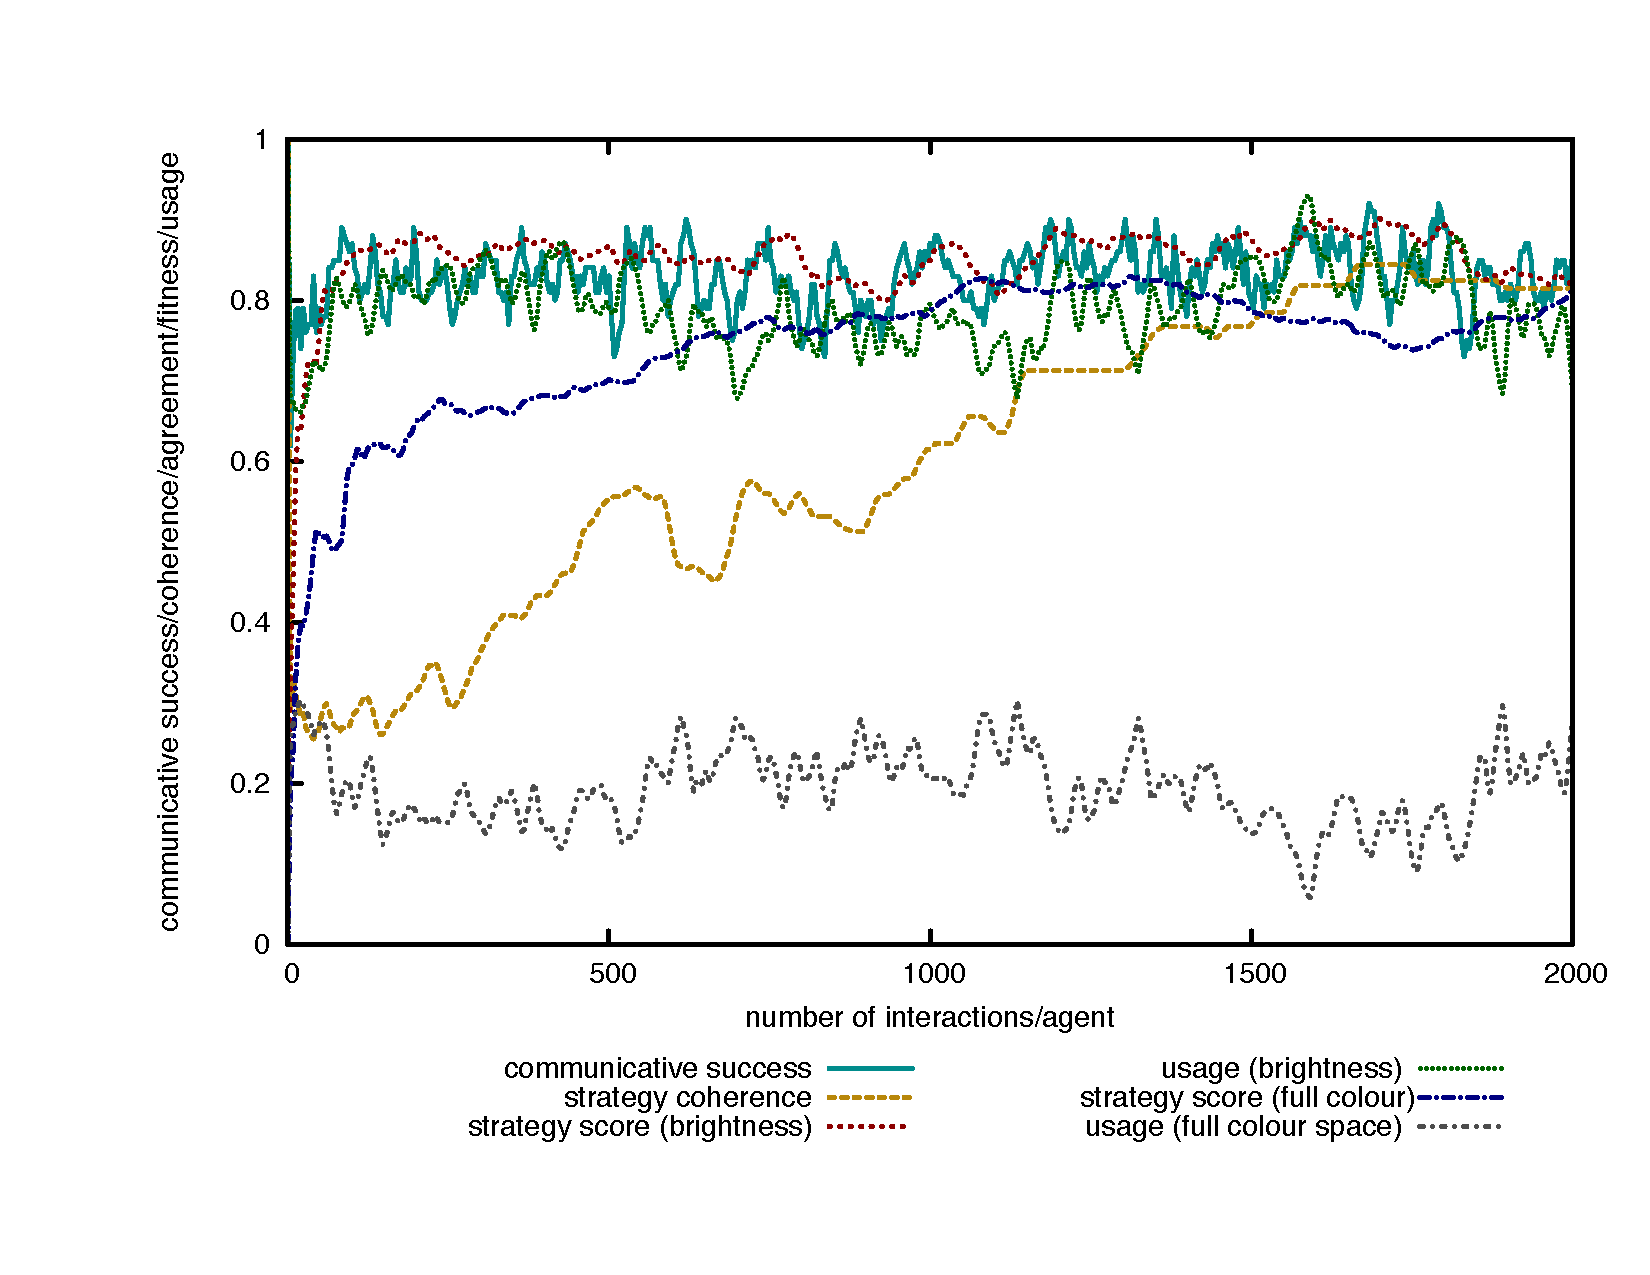
\includegraphics[width=.9\textwidth]{chap12/figs/strategies-one-winner.pdf}}
\caption{{Communicative success stays constant. The Brightness Colour Strategy becomes 
dominant very early due to random fluctuations. It stays dominant but barely. 
The strategy coherence (i.e. whether agents agree on the 
default strategy) increases gradually. The Full Colour Strategy remains still in use for cases where
it is needed. \label{fig:strategies-one}}}
\end{figure}

Rich and complex dynamics results from this general system. In the results shown in \figref{fig:strategies-one}, the 
set of prototypes is kept fixed, namely equal to the focal colours underlying 
the Spanish colour system, which can be used either for the Full-Colour strategy or for the Brightness strategy. 
For example, the word `morado' (`purple') can both be interpreted in the full-colour space and in the brightness space. 

Agents are initialised with a random value for the strategy-score for the Brightness-based versus
Full-colour based strategy. When the dynamics described here takes its 
course (which includes the shifting of prototypes by speakers and hearers to be maximally adapted to the 
contexts that are presented), we observe several possibilities. In one simulation run (see \figref{fig:strategies-one}), 
the brightness-based strategy becomes and remains dominant. It could have been the brightness 
or the full-colour strategy, depending on small fluctuations in the early stages. 
In another simulation run we see that one strategy becomes dominant first (in this case the brightness strategy) 
to be overtaken later by another strategy (i.c.\ the full-colour strategy), 
as attested in the history of English colour terms (see \figref{fig:strategies-dynamics}). 
The two strategies continue to co-exist. Brightness is still used in 
circumstances where this gives a higher chance of communicative success, for example when colour chips are 
close in hue but distinct in brightness or when there is a word which has most of its success in the brightness 
dimension. 


\begin{figure}[b]
\centerline{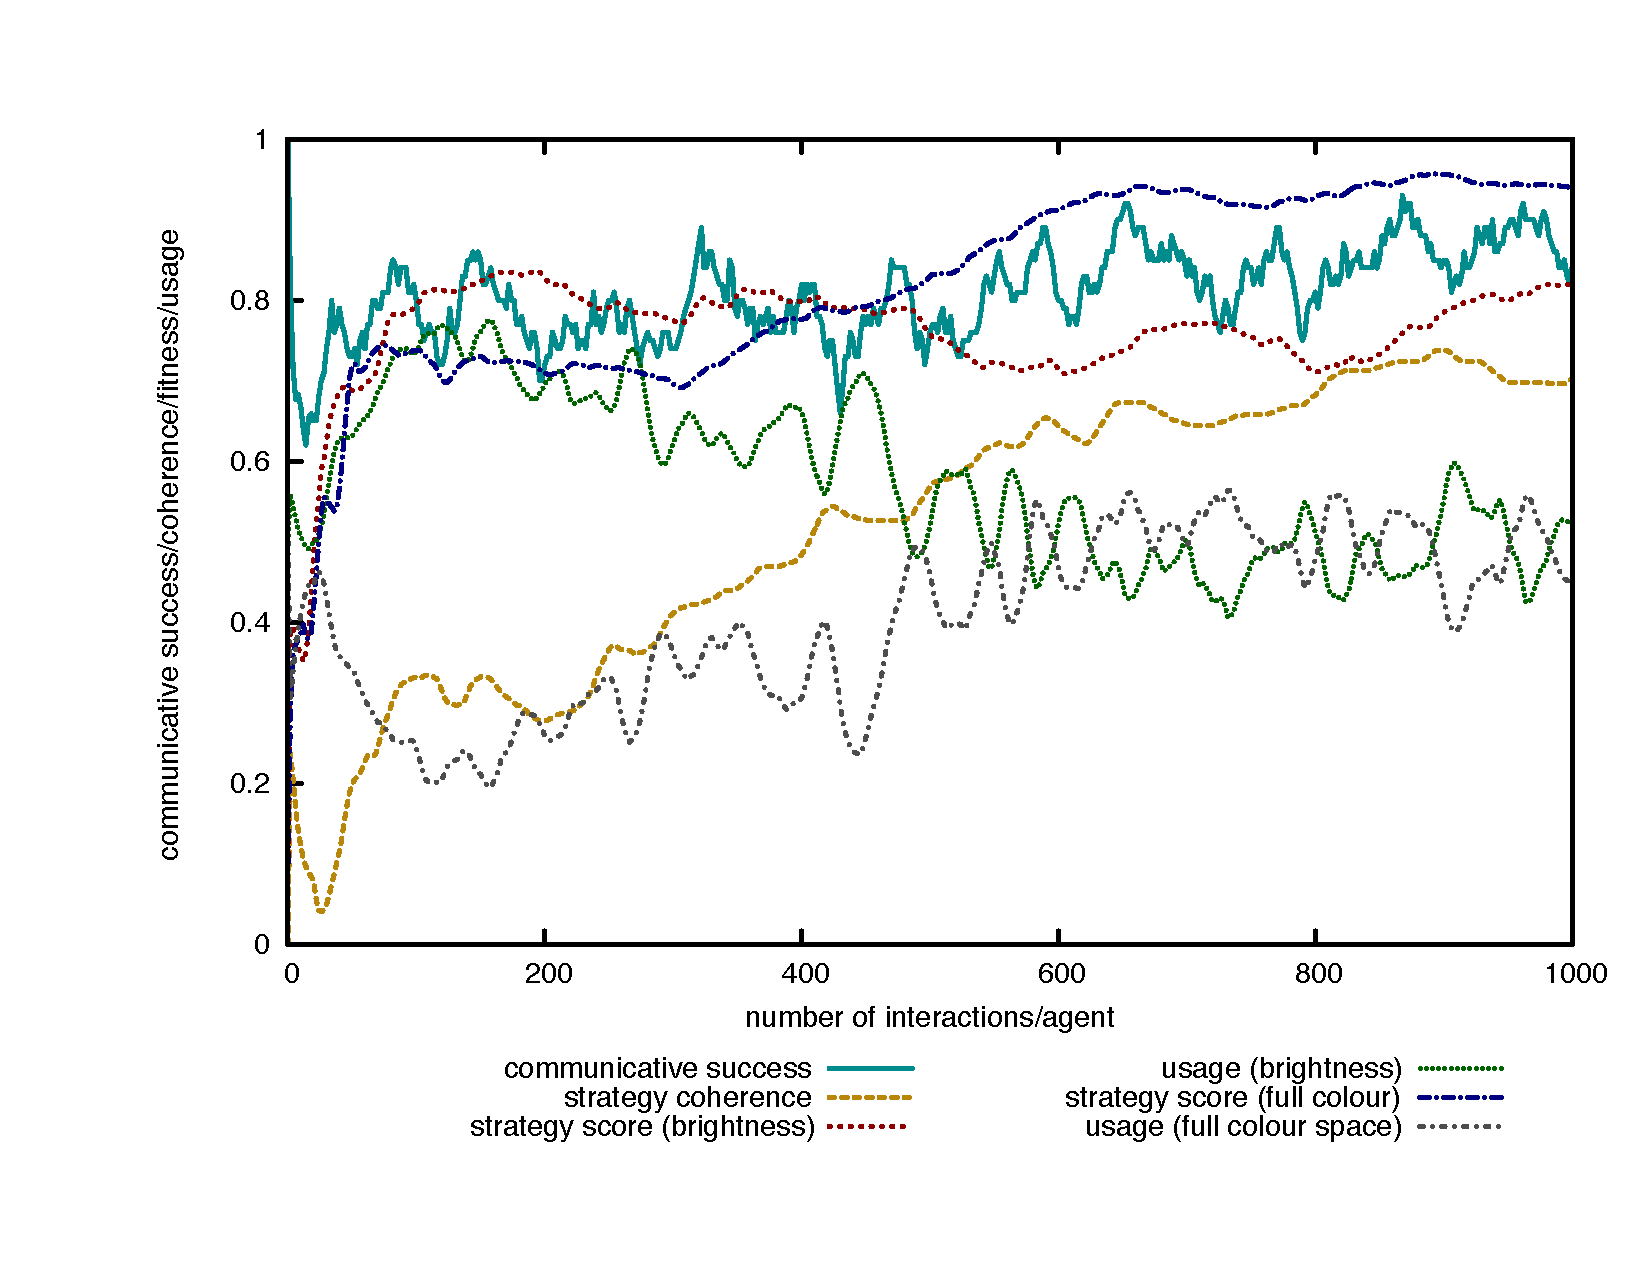
\includegraphics[width=.9\textwidth]{chap12/figs/strategies-competition.pdf}}
\caption{{Initially the brightness strategy is dominant, but then the full-colour 
strategy gradually takes over and becomes dominant around 400 games/agents. Strategy coherence within the population
progressively increases.}
\label{fig:strategies-dynamics}}
\end{figure}

\section{Generation of new strategies}

The previous section showed how there can be competition or cooperation between strategies, fought out through the 
performance of the language systems against the niche factors in which \is{strategy generation}
the language strategies operate. But a Darwinian evolutionary framework requires that there is not only 
selection and a self-enforcing causal feedback loop 
but also that new elements get generated, in this case new strategies, which can then be subjected to 
a selectionist dynamics. How can we explain that new 
strategies arise? This is the most challenging difficult question of evolutionary linguistics research and very much an 
open question. We basically have to move up to a meta-level where we have strategies for building 
strategies, further called meta-strategies. \is{meta-strategy} It is unclear whether they have to be innately given or 
whether they are themselves also the result of developmental processes and a cultural dynamics. 
There are two aspects to a strategy: a conceptual side and a linguistic side. For the conceptual 
side, solid results have been achieved using IRL, which was from the beginning developed to allow the generation of 
new conceptualisation strategies. So far a single meta-strategy has proven to be quite successful in this case. 
The linguistic side however is still to a large extent in a stage of fundamental research, and here there appear to 
be several different meta-strategies, used by different language communities. Each of these two aspects is now 
discussed.

\subsection{A meta-strategy for generating new conceptualisation strategies}
% {\bfshape A Meta-strategy for Generating new Conceptualisation Strategies}\\

As explained in the previous chapter, the conceptualisation of grounded meaning takes the form of programs which perform 
operations over the world model. For example, for the spatial domain, this amounts to
cognitive operations such as filtering the objects in the context with a particular prototype, geometric 
transformations to re-interpret the scene from a particular perspective, execute set operations, etc. We have seen that these 
programs can be formulated in terms of constraint networks. Each cognitive operation helps to determine or constrain
the value of slots and computation terminates successfully when all slots could be filled. 


\begin{figure}
\centerline{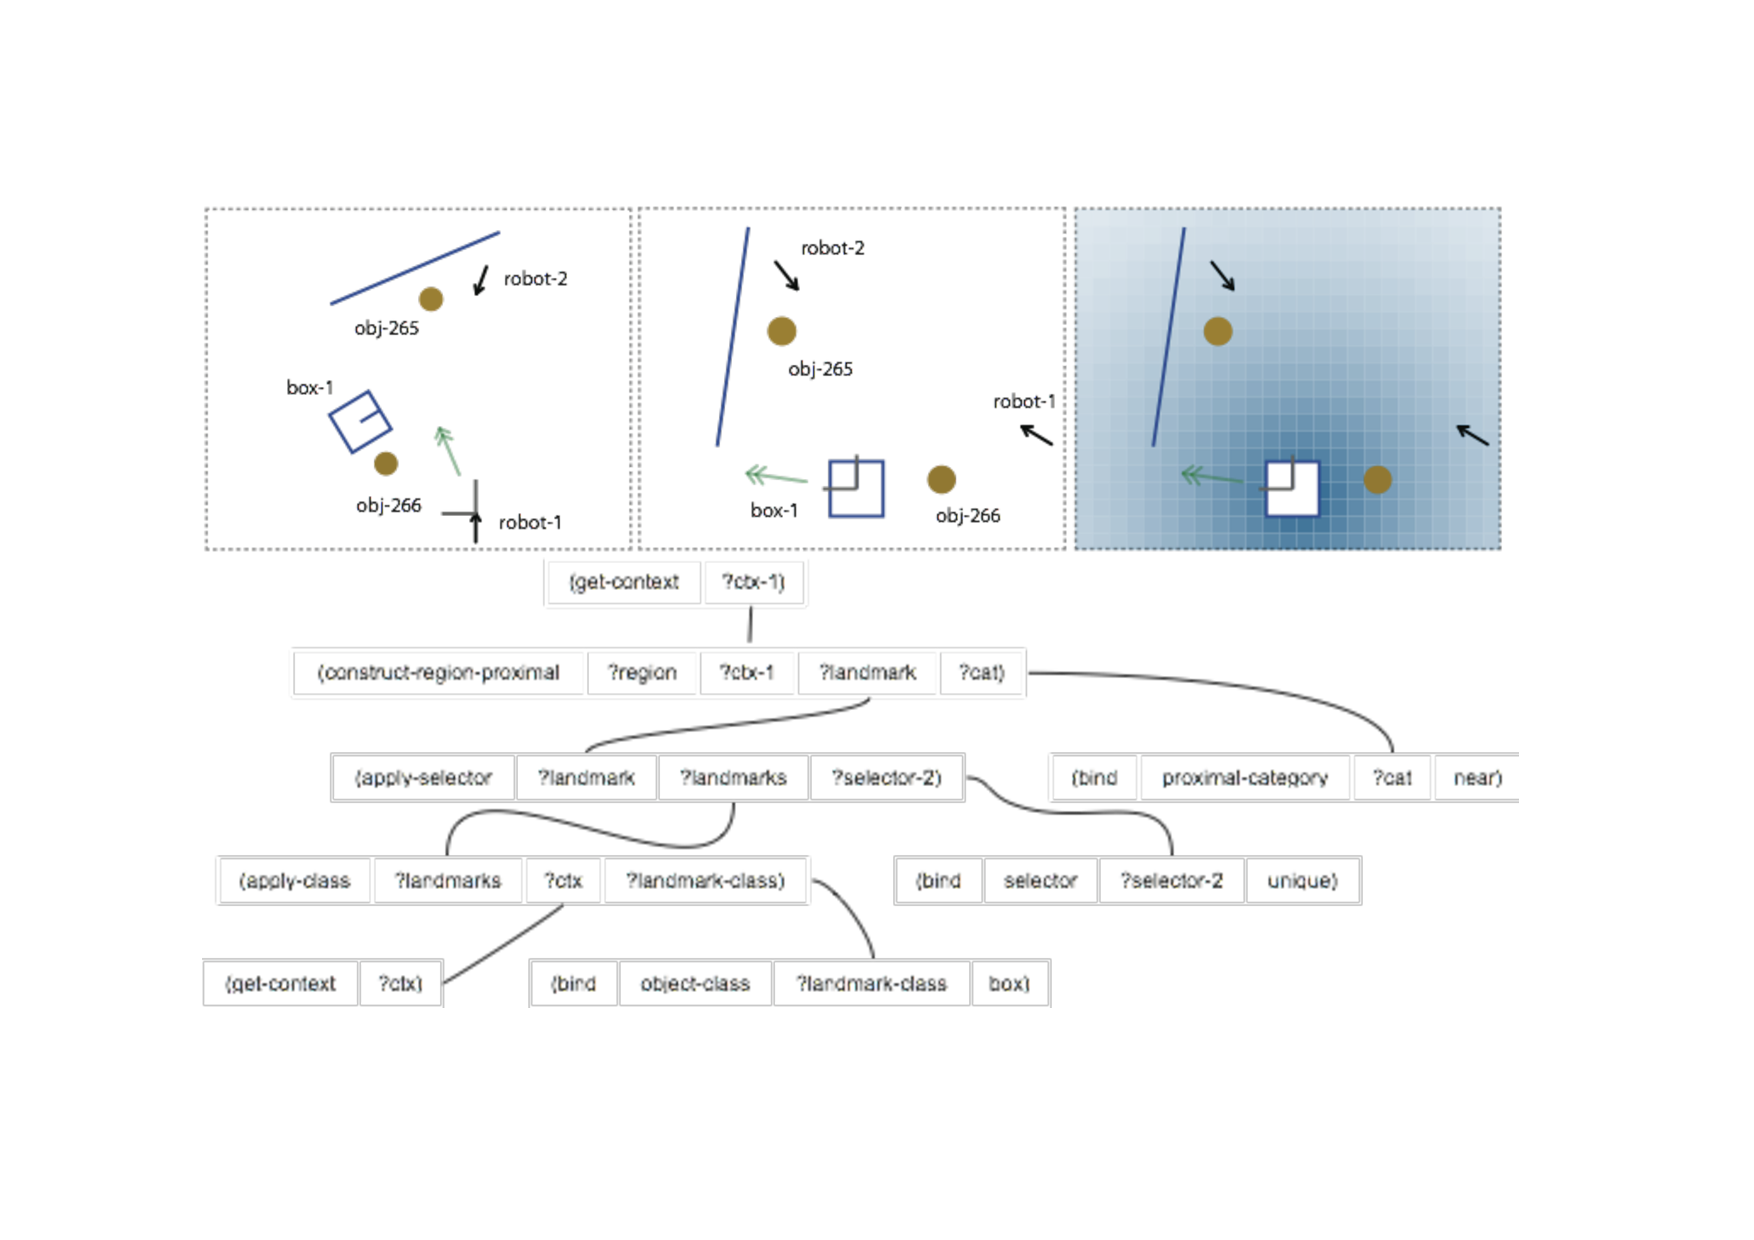
\includegraphics[width=.9\linewidth]{chap11/figs/near-the-box2.pdf}}
\caption{Example of a conceptualisation for the phrase `near to the box'. {\itshape Top:} 
Leftmost: The situation as perceived by the robot. Middle: situation after a geometric transform where the box is 
made the central perspective. Right: Area around the box which reflects (in terms of darkness of the colour) how 
near objects are to the box. {\itshape Bottom:} IRL constraint network for this conceptualisation.
\label{fig:spatial-strategies}}
\end{figure}

We will use the domain of spatial language again as a source of examples, based on experiments carried out by 
Michael Spranger. It uses the \textsc{qrio} humanoid robots 
and scenes like the one shown in \figref{fig:spatial}. An example of a constraint network from this domain 
is shown in \figref{fig:spatial-strategies}. It is the network for the phrase `near the box'. `Near' is a proximal 
relation which categorises objects in terms of how near they are to a landmark (in this case the box). In a list form the 
network looks like this: 
\begin{small}
\begin{verbatim}
1. (get-context ?ctx-1) 
2. (construct-region-proximal 
    ?region ?ctx-1 ?landmark ?cat) 
3. (bind proximal-category ?cat NEAR) 
4. (apply-selection ?landmark ?landmarks ?selector-2)
5. (apply-class ?landmarks ?ctx ?landmark-class) 
6. (bind selector ?selector-2 UNIQUE) 
7. (get-context ?ctx) 
8. (bind object-class ?landmark-class BOX)
\end{verbatim}
\end{small}
The order of these operations does not matter as values propagate and constraints become active until no further progress
can be made. Operations in 4, 5, 6, 7 and 8 provide the referent of `the box'. The following contributions 
can be made by each of the cognitive operations: The predicate \textsc{box} gets bound to ?landmark-class in operation 8. Object-class is 
the type of ?landmark-class. The context, i.e. all objects in the present situation, gets bound to ?ctx in operation 7. 
The selector \textsc{unique} gets bound to ?selector-2 in operation 6. 
Then the operation apply-class is applied to all the objects in ?ctx (the context) to find the possible landmarks which 
get bound to ?landmarks using the ?landmark-class (\textsc{box}). This set is assumed to be a singleton and so 
in operation 4 the unique element in the set of ?landmarks can be selected 
and bound to ?landmark. 

\enlargethispage{1\baselineskip}
The remaining three operations apply the proximal relation. In operation 3 ?cat is bound to the proximal-category \textsc{near}. 
In operation 1, ?ctx-1 gets bound to 
the context. And finally in operation 2, the region around the landmark, which satisfies the category ?cat (\textsc{near}), can 
be computed and bound to ?region by ``construct-region-proximal''. The construction-region-proximal constraint has to perform first 
a geometric transformation on the scene, constructing a world model from the viewpoint of the landmark, i.e. the box. 

A {\itshape conceptualisation strategy} is an abstraction of such a concrete conceptualisation network. 
\is{conceptualisation strategy}
It consists of a network that acts as a useful chunk and is therefore a modular unit that can be linked into a larger network. 
The chunk has a set of open variables with which the network can be linked to other networks. 
For example, the network shown in \figref{fig:spatial-strategies} can be made more abstract to handle many instances 
of proximal relations, not only `near the box', but also `far from the box', `close to the box', `near the boxes', 
`near the table', `very far from the wall', etc. 
The open variables are ?cat, ?selector-2, and ?landmark-class, which have to be supplied by lexical items or 
phrases. The network is then as follows, with operations at 3, 6 and 8 removed: 
\begin{small}
\begin{verbatim}
1. (get-context ?ctx-1) 
2. (construct-region-proximal ?region ?ctx-1 ?landmark ?cat) 
4. (apply-selection ?landmark ?landmarks ?selector-2)
5. (apply-class ?landmarks ?ctx ?landmark-class) 
7. (get-context ?ctx) 
\end{verbatim}
\end{small}
The network has to be completed with bindings for the open variables, but all the other variables can be 
computed through the network itself. 
Network-chunks are expressed through a grammatical construction, which expresses which chunk is involved 
and how the initial values of the slots are to be expressed. In this 
case it is a noun-phrase construction, syntactically of the form [noun preposition article noun] and 
semantically constrained as [proximal-category selector object-class]. 

Spranger demonstrated how new spatial conceptualisation strategies can be derived. The process uses the regular 
way in which the speaker agent finds possible conceptualisations, namely through a search process (\figref{fig:tree}). 


\begin{figure}
\begin{centering}
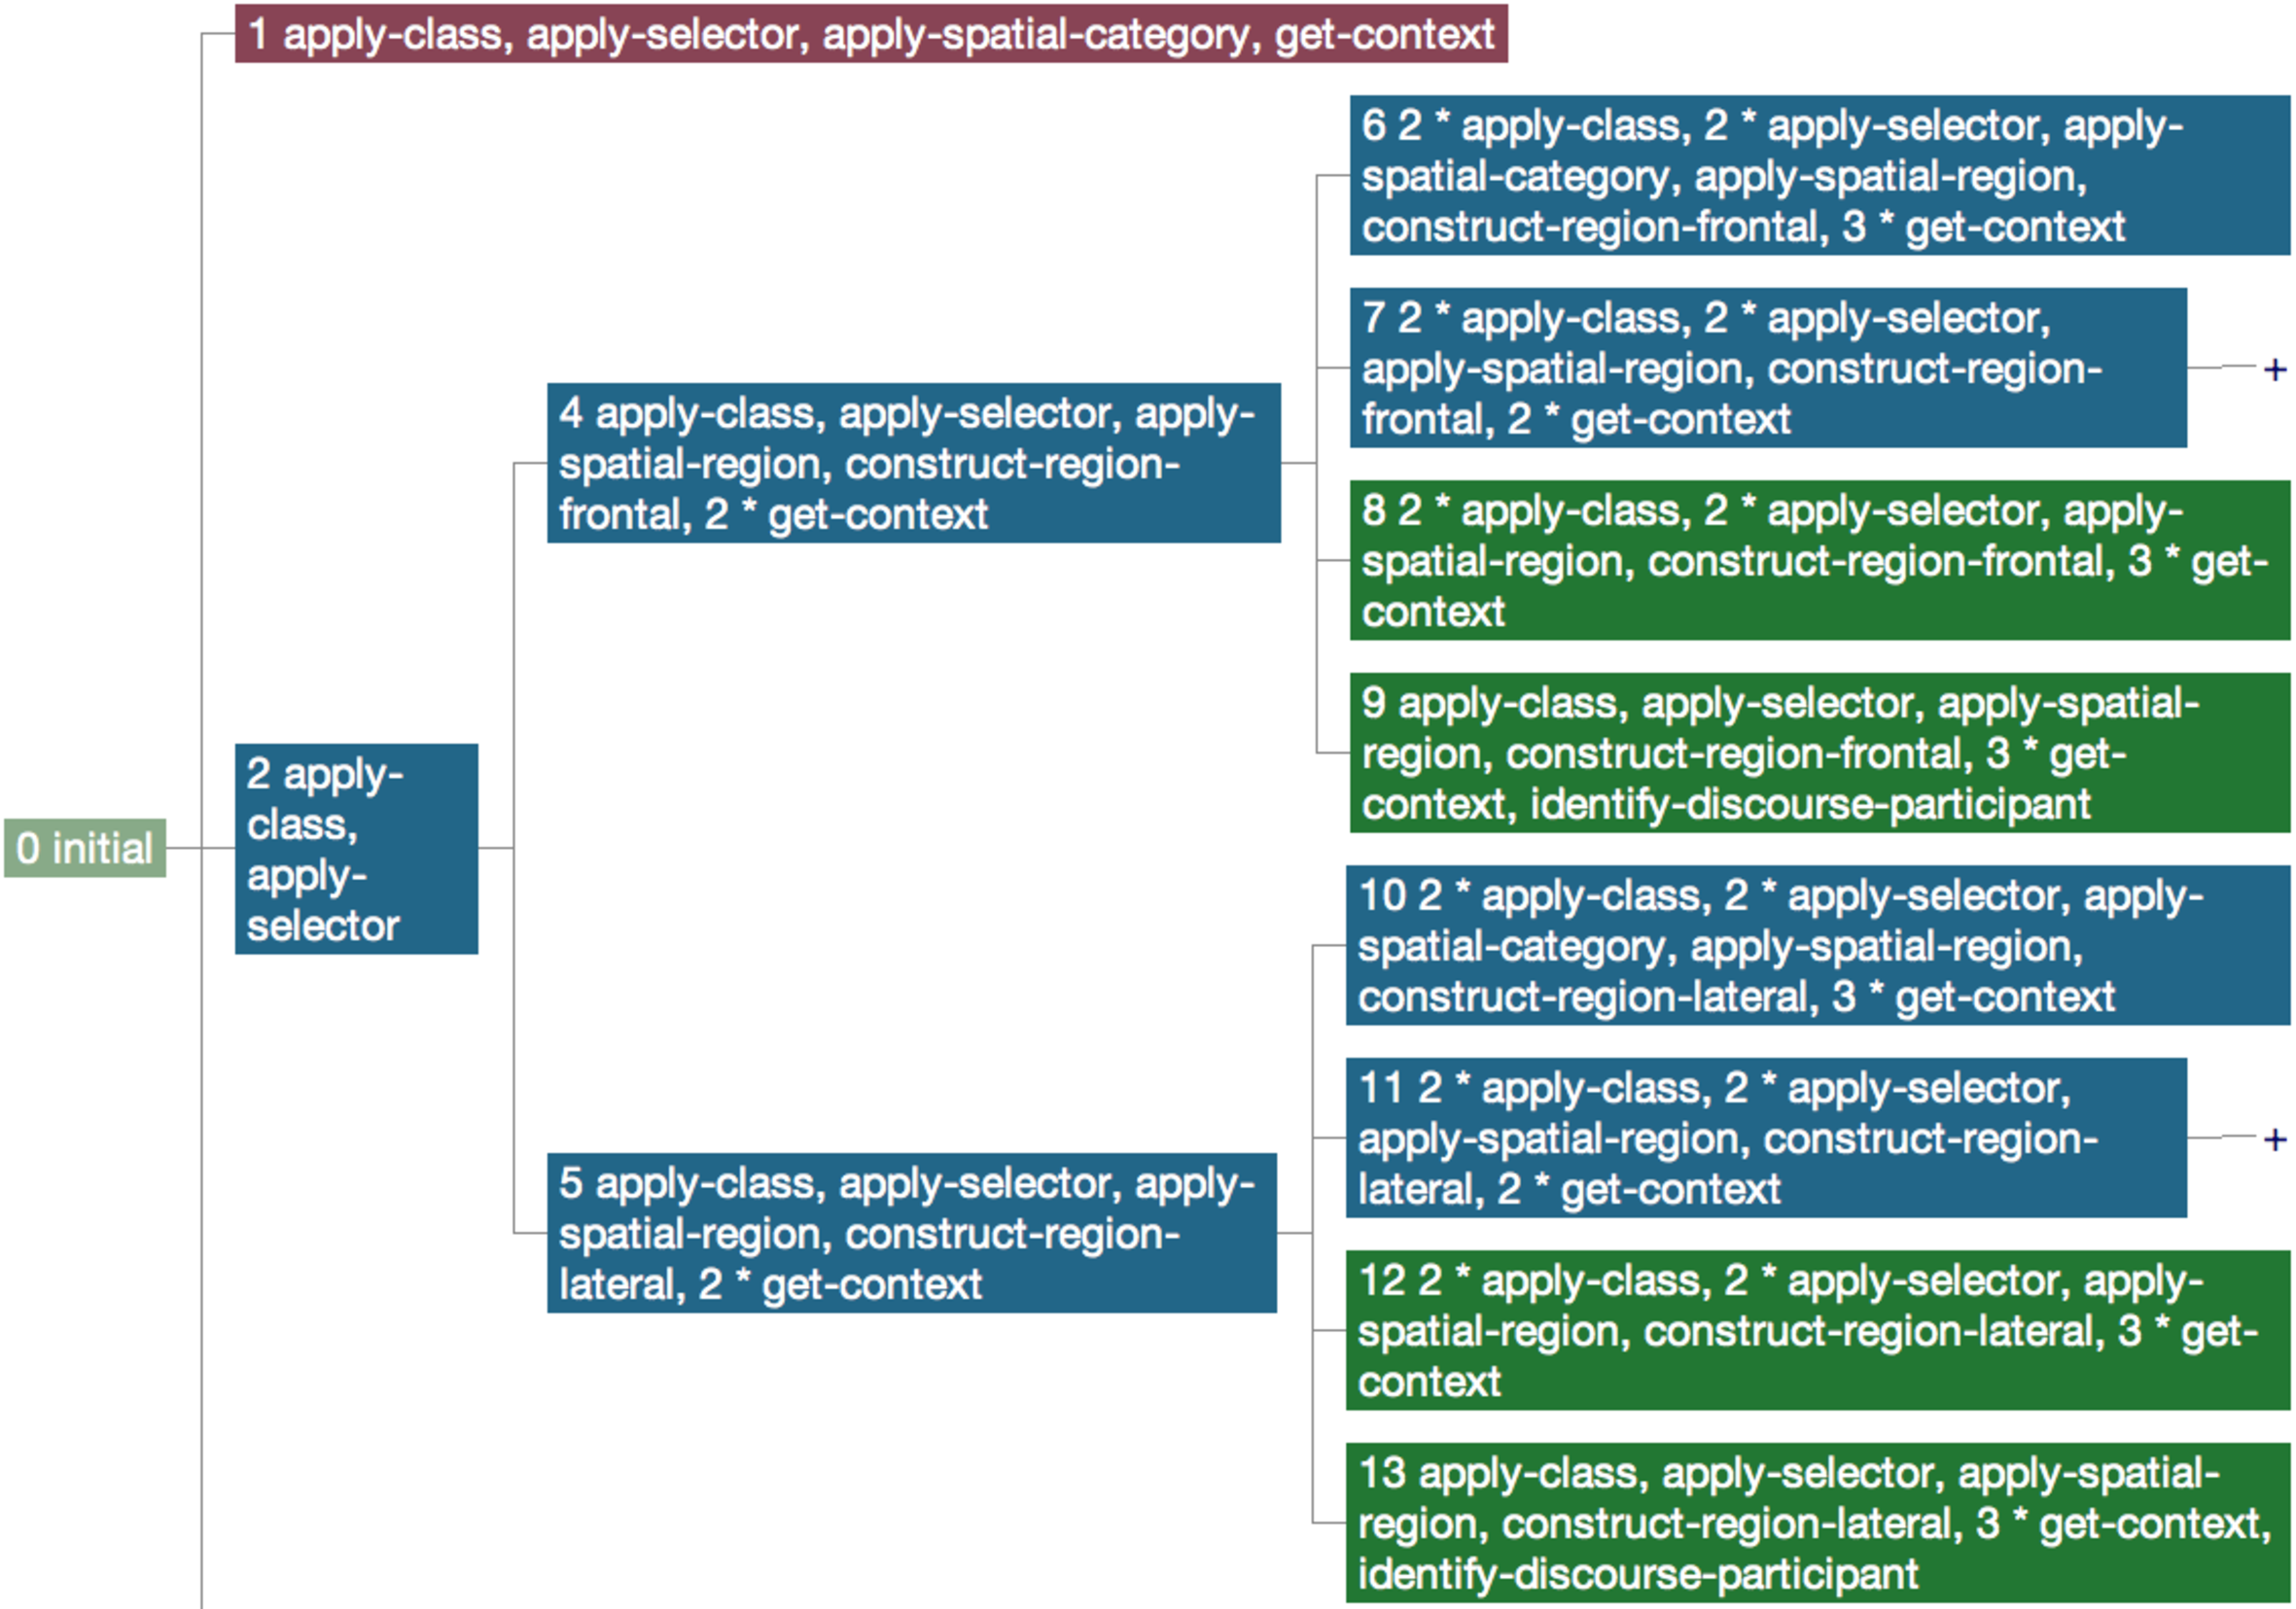
\includegraphics[width=1\columnwidth]{chap12/figs/conceptualization.pdf}
\end{centering}
\caption{The meaning of an utterance is found through a search process, starting from an empty network, progressively more 
constraints are added until a solution network is found that, when executed, yields the topic chosen by the speaker.}
\label{fig:tree}
\end{figure}
\enlargethispage{1\baselineskip}
As explained in the previous chapter, the speaker starts from a particular communicative goal (the topic) within a 
specific context. Each step in the search process adds progressively more nodes and at each step, the network is tried out to 
see whether it is able to compute anything in the present context and whether it brings the 
speaker closer to a possible effective conceptualisation. The end-nodes of the search tree contain either networks that 
do not yield a solution or a network that is a possible conceptualisation offered for translation into an utterance. 

Often there is more than one solution. (There are already four solutions in the tree in \figref{fig:tree} and more solutions 
would turn up if some of the nodes are worked out further.) Solutions are ranked based on various criteria such as their 
complexity, the score of the prototypes involved, or how well they can be translated into an utterance.

Once an adequate conceptualisation is found and it leads to a successful game, modular sections of the network can be 
abstracted and used as the basis of reusable conceptualisation strategies in the future. Each conceptualisation 
strategy has its own score which is updated using the lateral inhibition dynamics as used for 
the lexical or grammatical constructions as explained in earlier chapters. The frequency of use and success 
of a strategy depends partly on whether the ``niche'' in which a strategy is most effective occurs frequently, partly 
on what is preferred by the rest of the population, and other criteria such as complexity.


\begin{figure}
\begin{center}
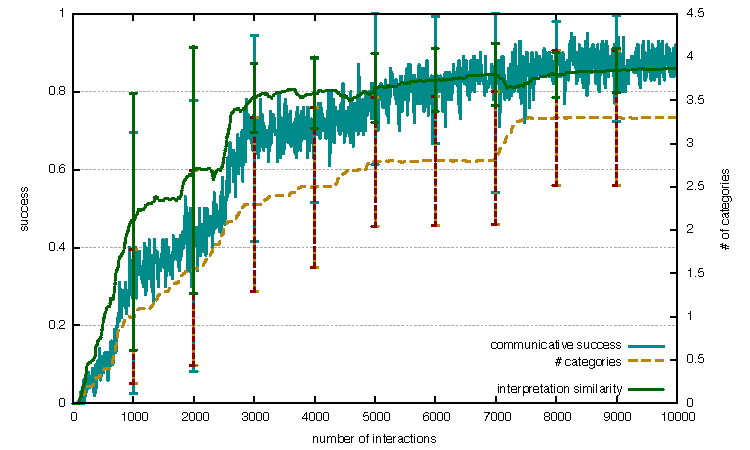
\includegraphics[width=\textwidth]{chap12/figs/chunk-alignment-category-invention-success.pdf}
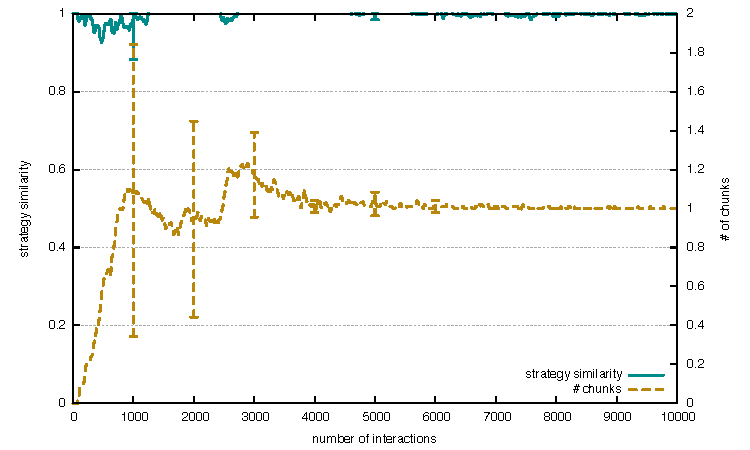
\includegraphics[width=\textwidth]{chap12/figs/chunk-alignment-category-invention-alignment.pdf}
\caption{This experiment combines strategy invention, alignment, and category development by each strategy. The top figure
shows language games on the x-axis, and communicative success, average 
number of categories, and interpretation similarity on the y-axis. The bottom figure shows the similarity between 
strategies and the average number of strategies in the population. One strategy becomes dominant.}
\label{fig:all}
\end{center}
\end{figure}

\figref{fig:all} shows an example experiment in which all the aspects discussed in this section are brought together. 
A population of 10 agents is developing new conceptualisation strategies for a niche that encourages preference 
for a particular strategy, namely a projective strategy with possible perspective reversal, as in `the box in front 
of the wall'. We see that communicative success steadily rises and that the number of 
spatial categories increases. The bottom graph zooms in on the conceptualisation strategies. We see that agents reach 
a consensus about a dominant strategy after a period in which new strategies 
are invented and tried out. 

\subsection{Meta-strategies for generating new lexico\-gram\-matical strategies}
% {\bfshape Meta-strategies for generating new lexico-grammatical strategies}\\ 

Are there general meta-strategies that can be used to generate the kind of lexico\-gram\-mat\-ical strategies 
that can in turn generate all the language systems we observe 
in today's languages? This is a very profound question, related to the ongoing debate in linguistics on the existence of 
a universal language acquisition device. A lot of ink has been spilled but we need to do profound computational modelling 
of meta-strategies and thorough experiments to find out. 

Generally speaking, a lexico-grammatical strategy has two components: {\itshape diagnostics} which monitor how 
language processing is going and {\itshape repairs} which add new 
constructions to the agent's inventory. 

For {\itshape lexical strategies}, the diagnostics consist in checking whether there is part 
of the meaning that is not yet covered by any lexical item. The repair then consists in introducing 
a (possibly new) word and introducing a new lexical construction for this word. 
This strategy is already used by the Talking Heads. When part of a meaning cannot be covered, a new word form is randomly generated
and used from then on for this meaning, but possibly in competition with other words that were later acquired for the same 
meaning. 

\newpage
A study of ongoing change in the vocabularies of human speakers shows that the invention of a brand new word form happens seldom. 
Usually an existing wordform is recruited to express an uncovered meaning. The meaning of the already existing word form
expresses aspects of the novel meaning to be expressed but there is not an exact overlap. However, the existing word is sufficiently 
suggestive so that the hearer can guess what meaning is intended by the speaker. For example, the word `mouse' becomes 
adopted for computer mouse based on its appearance. Often a compound of several words is used, each of them suggesting 
other aspects of the meaning, such as `bitcoin', which suggests digital (`bit') and currency (`coin').  
There are several other strategies, for example, an abbreviation of a long word becomes itself a single new word, 
such as `MOOC', meaning `massively open on-line course' and now standing for a course made available through the internet. 
There are also playful variations created with existing words, as for example
`wackadoo' which means `bizarre person' and probably originally came from the word `wacky'. 

\enlargethispage{1\baselineskip}
It is not really possible to capture the enormous creativity of human word creation in computational simulations 
because that would involve components for common sense inference and access to massive cultural knowledge. 
However we can do experiments to understand how new words may arise by analogy with existing words 
and how the meaning of words can develop further, for example by abandoning some of the aspects of 
the original meaning or gaining new meanings. Such experiments have 
been carried out in particular by \cite{Wellens:2008}. \is{flexible word meaning}


\begin{figure}
\begin{center}
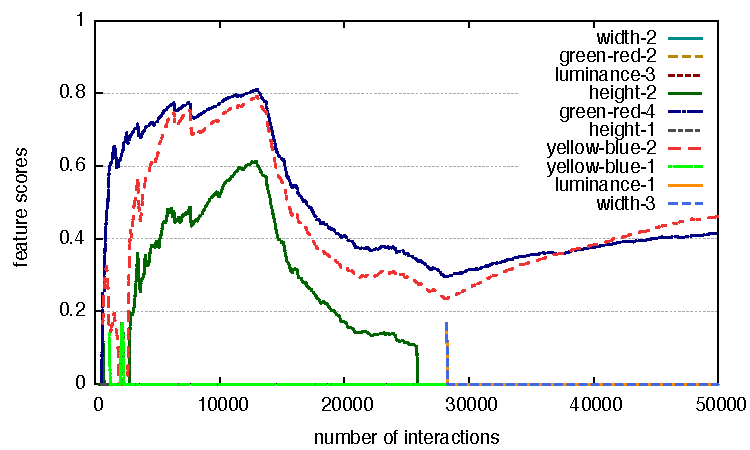
\includegraphics[width=\textwidth]{chap12/figs/attribute-scores-4.pdf}
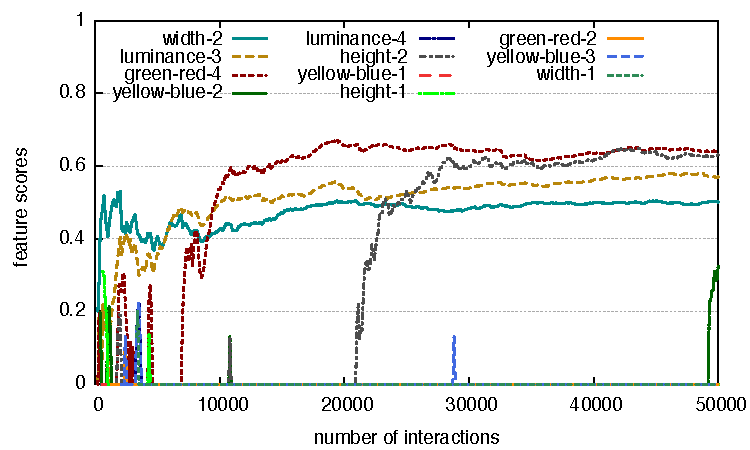
\includegraphics[width=\textwidth]{chap12/figs/dog-meaning.pdf}
\end{center}
\caption{Two examples of the meaning of words in terms of a set of component features whose weight can change over time.}
\label{fig:weightchange}
\end{figure}

In their ``adaptive, flexible word meaning strategy'', Wellens and Loetzsch assumed that the association between 
a word and the different components of the meaning (called its features) is flexible. Each component feature has a score and not 
all features have to be present in order to use a word. The scores of the features are updated depending on the success of the 
word and whether they were relevant in the situation in which the word was used. As a consequence we get a much more 
fine-grained dynamics in which the meanings of words may flexibly shift and a word may come to be used for another 
constellation of features that is only partially matching. \figref{fig:weightchange} shows examples of how these features 
evolve over time. They show the kinds of progressive shifts in meaning that we also observe in human lexicon evolution and 
demonstrate how words can come to be used for quite different meanings than their rigid original sense would demand. 

{\itshape Grammatical strategies} come in two types. There are first of all strategies that express additional meaning using 
syntax. The syntax can either take the form of ordering of the words, as in the distinction between an affirmative sentence
and a question, signalled by the use of the auxiliary `do' and inversion of the main verb and the subject (as in 
`Does he come?' versus `he comes'), or by the use of syntactic structure and function words, as in the verb phrase. For example, 
a phrase like `will have been coming' involves a future perfective using the auxiliary `will', the infinitive auxiliary (`have'), the 
past participle auxiliary (`been'), and the present participle main verb (`coming'). 

There are also strategies that focus 
on minimising the cognitive effort of the listener by signalling how words in the sentence need to be semantically grouped together. 
This happens generally in two ways: 

\begin{itemize}
\item Language-dependent markers for various syntactico-semantic features, such as number, gender, case, are introduced 
and the different words which need to be grouped are all marked for the same features. An example of this kind of 
grammatical agreement is `la belle fille' (French: the beautiful girl) where the article `la' and 
the adjective `belle' are both marked as singular feminine. 
\item The second strategy is phrase structure. Words are grouped together that are about the same object, 
a sequential order is imposed on these words, and patterns of orderings based on syntactic and semantic categories are
introduced. 
\end{itemize}
Extensive empirical work on grammaticalisation \is{grammaticalisation}
has given us a wealth of data how these strategies play out in the history 
of human languages.\footnote{
See for example: \cite{Heine:2007}, \cite{Hopper:1993}, \cite{Lehmann:1982}, \cite{Traugott:2013}.}
And the key challenge for evolutionary linguistics is to model 
these processes, the same way evolutionary biologists model speciation or species evolution. 

I here just point to one series of experiments, I conducted with Katrien Beuls, on the origins of agreement 
systems, which follow the latter strategy \cite{Beuls:2013}. The challenge was to discover by 
what kind of language strategies an agreement system could arise and to identify the basic building blocks with which 
evolutionary experiments could be set up. \is{grammatical agreement}

Historical linguists have researched many concrete examples of how agreement systems arise.\footnote{See for example: \cite{Lehmann:1988}, \cite{Luraghi:2011}.}
There are invariably the following phases: 
\begin{enumerate}
\item Agreement markers derive from reusing existing words, such as pronouns or classifiers. 
\item The markers derived from independent words become shorter, they lose part of their form, 
then become clitics and later affixes. For example, the Dyirbal (Australian aboriginal)
agreement marker {\itshape m-} evolved from the classifier {\itshape mayi}, which means 'non-flesh food'. 
\item The features that agreement markers express, which are initially semantically 
grounded, invariably become more abstract and get to be used in 
a purely conventional manner. For example, the masculine/feminine 
gender distinction has its basis in male/female sex, but is then arbitrarily applied to inanimate objects, so that table 
might be masculine in one language (German: {\itshape der Tisch}) but feminine in another (French: {\itshape la table}). 
\end{enumerate}
Starting from a game of reference, similar to the Talking Heads experiment, populations of agents were programmed 
first to build a ``formal'' agreement system, i.e. a system based on formal markers without any meaning, and then 
a meaningful grammatical system, with grammatical markers that express semantic features. The experiment was 
then extended with further strategies that optimise three niche factors:
\begin{enumerate}
\item The recruitment of existing words as markers makes the acquisition of new markers more accurate because it is based 
on existing words and so the meaning can be guessed more easily. This helps to propagate the markers faster in the population. 
\item The phonological reduction of word forms leads to less articulatory effort, as we have already seen with the German 
article system. 
\item Conventionalisation leads to a smaller inventory, and hence less memory requirements and better preservation of the 
language system. 
\end{enumerate}

Here I just show results for one example, the phonological reduction strategy. 
\is{phonological reduction strategy} Although sophisticated models of speech articulation
exist and they predict the kind of errors and variations that speakers tend to introduce and 
how they influence sound change, we have used a simpler model that nevertheless brings out the language dynamics
clearly. Speakers optimise articulation by leaving out the last consonant or vowel of a marker with a certain probability $\epsilon=0.1$. 
Hearers are flexible enough in their parsing of markers to 
recognise that a truncated form is a variant of an existing marker, as long as it deviates 
for only one consonant or vowel.
When an agent produces or encounters a truncated marker, he stores it in his inventory as a new variant of the original 
marker, and later uses the original or the truncated form with equal chance. 
However, as soon as an agent encounters the truncated marker for a second time, he adopts it as the 
new norm and the old form is discarded. 
It is possible that the agent encounters again the previous older form which may then be re-adopted and reused if it is encountered 
more than once. However, at some point, there are enough agents using the new variant so that the whole population shifts in a phase transition. 

\begin{figure}
\centerline{i) 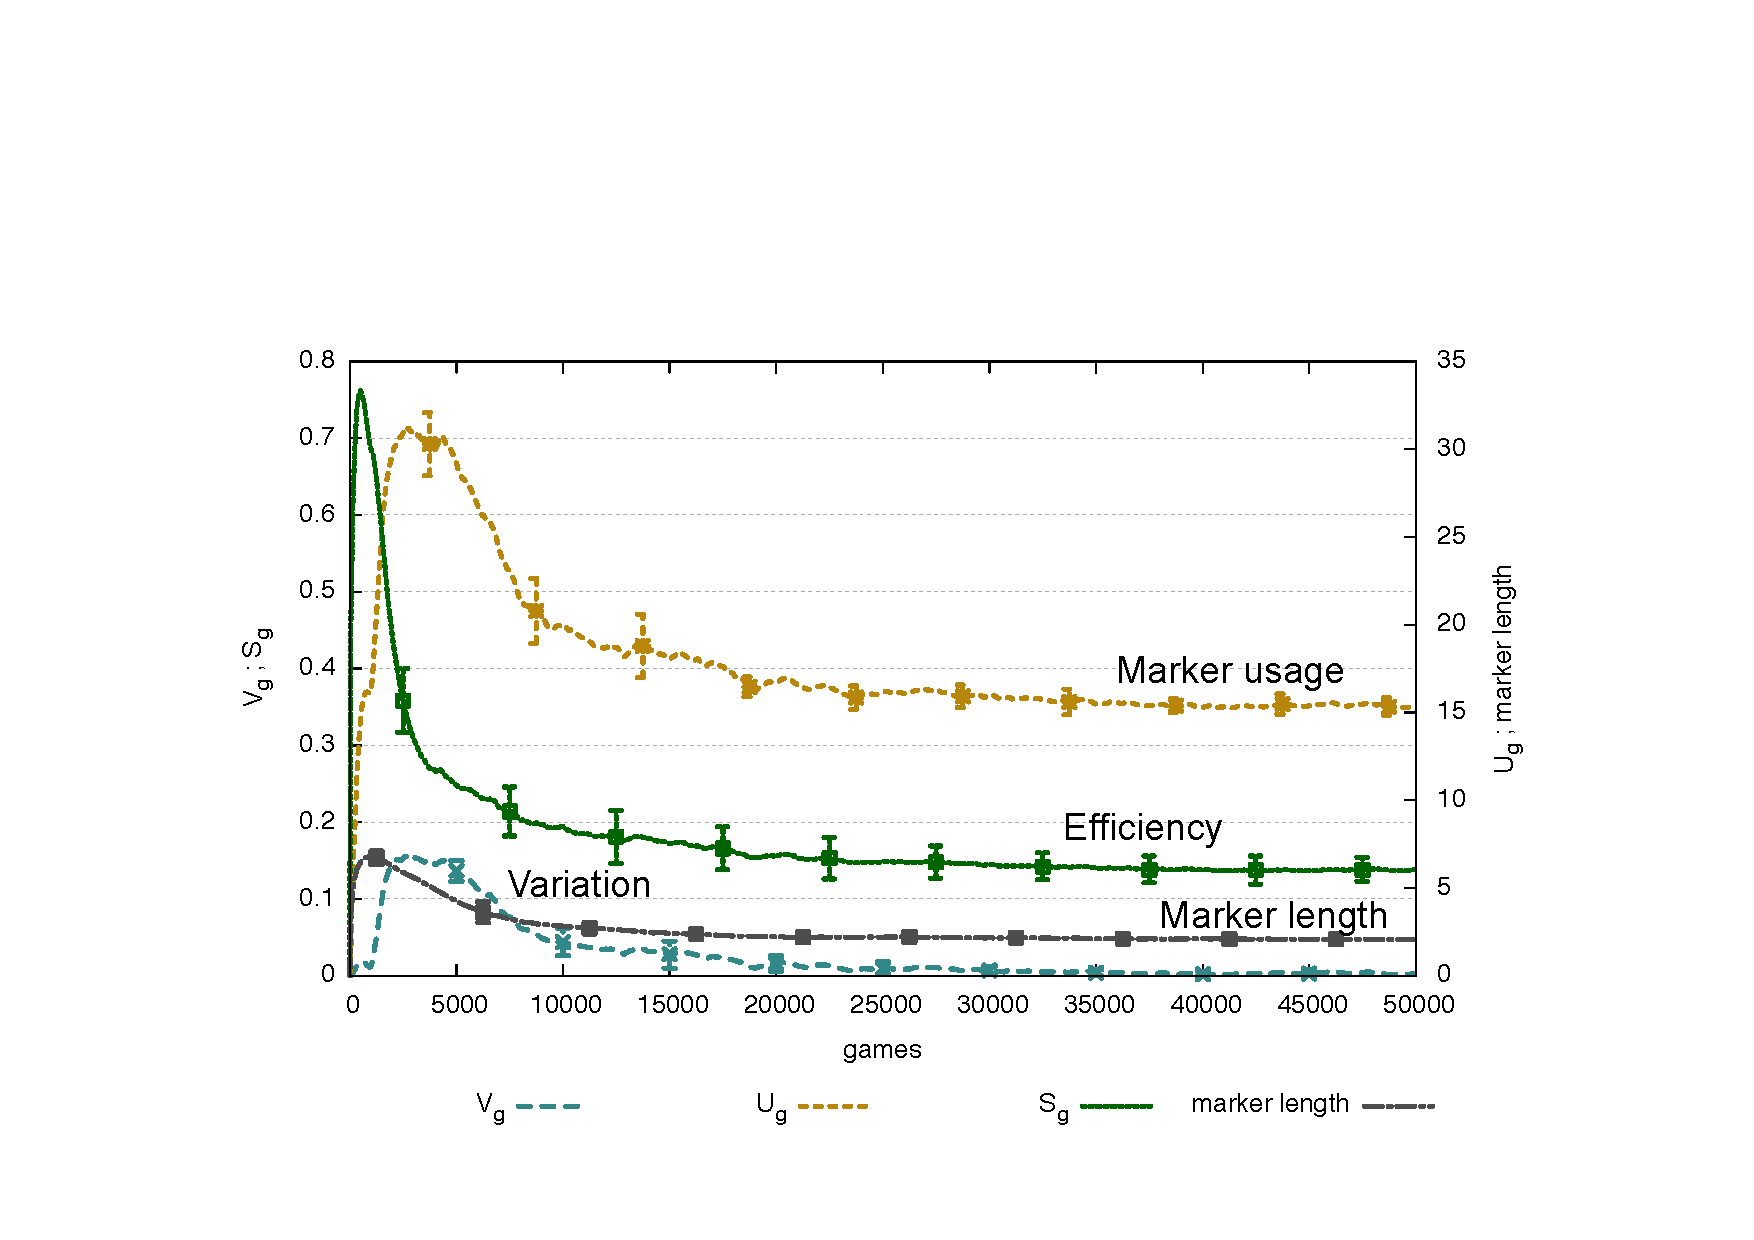
\includegraphics[scale=.5]{chap12/figs/erosion-performance-summary.pdf}} % fig14-i-erosion-performance
\centerline{ii) 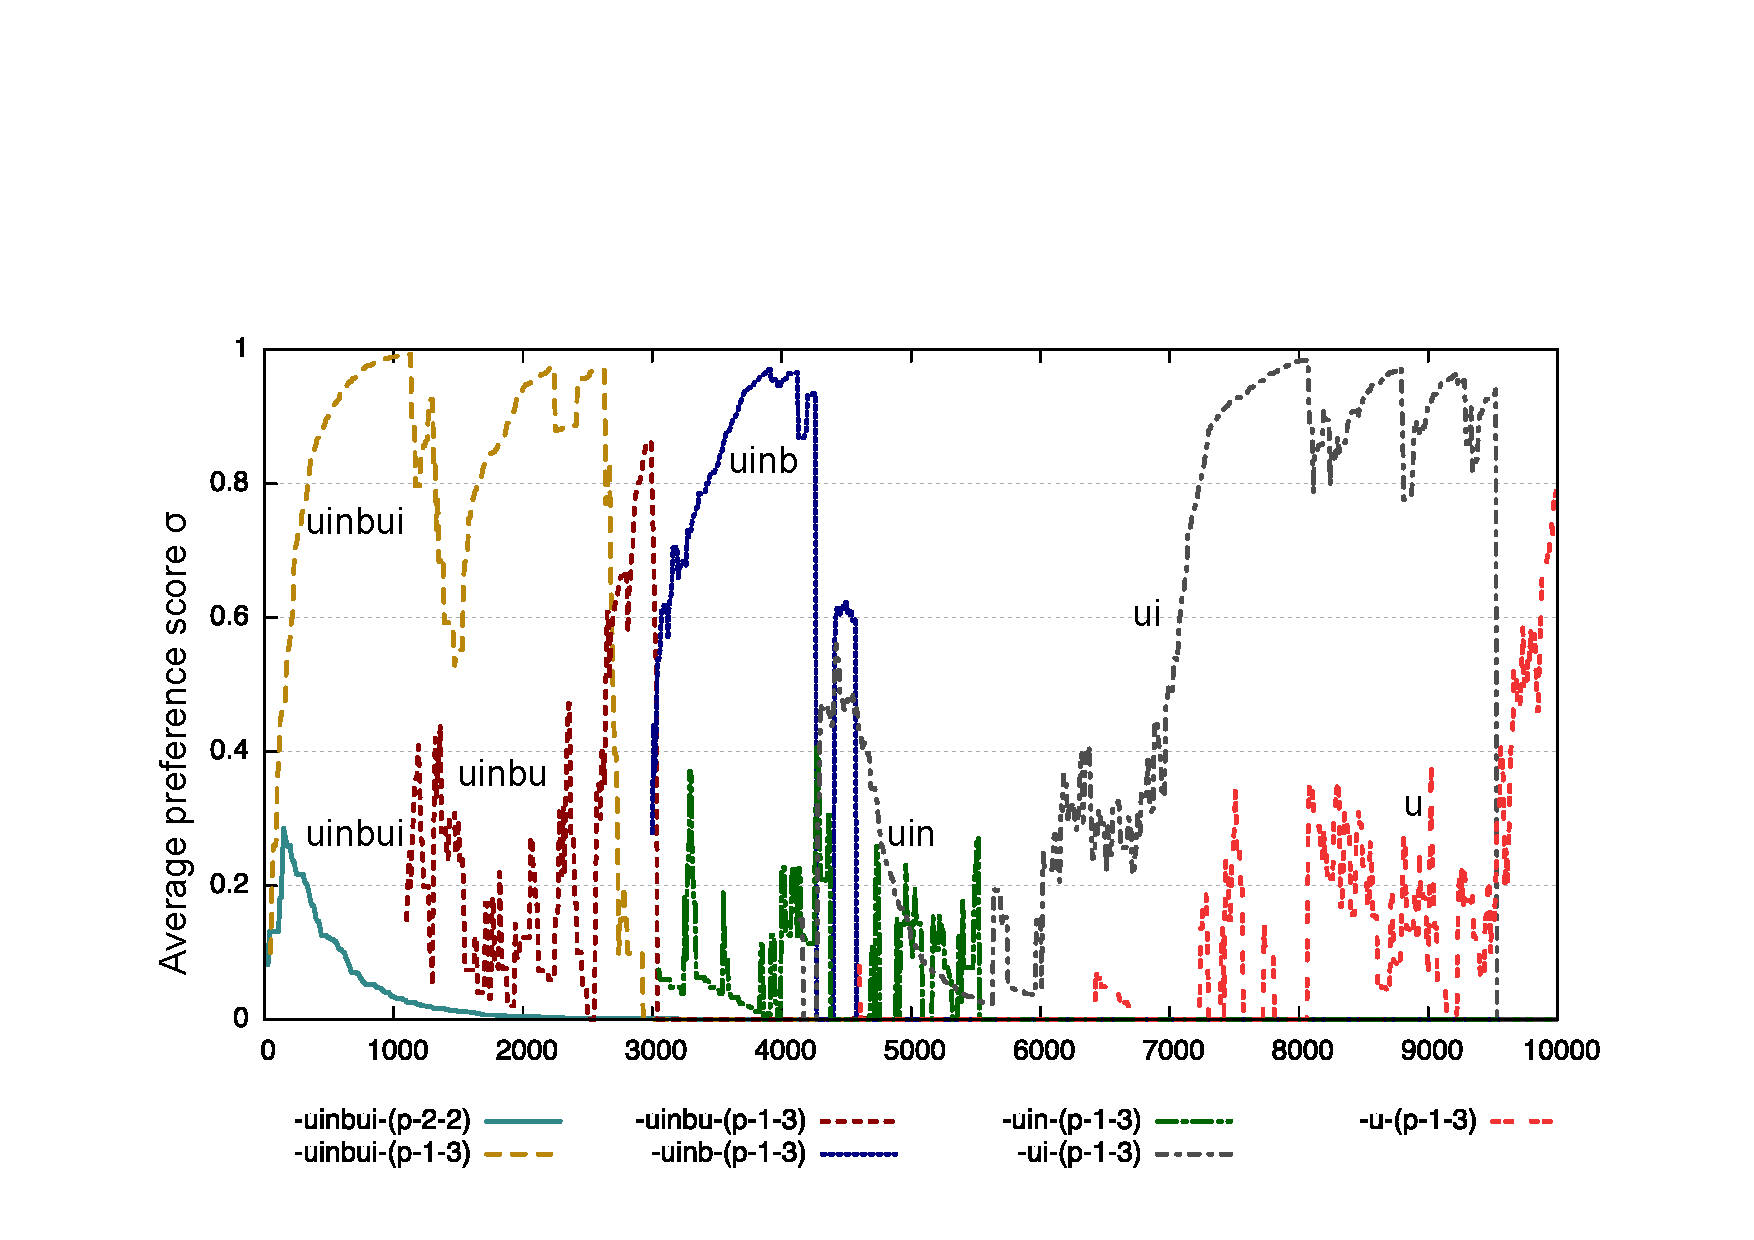
\includegraphics[scale=.4]{chap12/figs/uinbui.pdf}} % fig14-ii-uinbui
  \caption{{Performance of the phonological reduction strategy.} i) Average performance values
for 50 game series for a total of 50,000 games (average of 10,000 per agent). We see that the length of the markers progressively 
diminishes, thus reducing articulatory effort, 
but variation $V_{g}$ does not increase, implying that the system is stable. The marker inventory size remains constant as well.
ii) Trace of the changes to a marker in a single
experiment. The marker {\itshape -uinbui} erodes progressively to {\itshape -u}. A truncated variant is typically present for 
a while in the population until a phase transition happens and it becomes dominant.}
  \label{f:erosion}
\end{figure}

\figref{f:erosion} shows the outcome of a computer simulation of this phonological reduction strategy. An agreement system based on meaningful markers is emerging using the meaningful marker strategy. But after agents reach a stable level of performance
(in the experiment this is typically  
after 200 games per agent), they occasionally introduce phonological reductions with probability $\epsilon=0.1$ 
and this leads to the erosion 
of the original markers. \figref{f:erosion} top) shows that the average marker length is decreasing from an 
average of 7 to 4 consonants and vowels, without affecting performance. There is greater variation $V_g$ in 
the population because there are 
always different variants of the same marker in use, but this generally does not 
have an impact on communicative success because agents are able to recognise them as a variant of their own norm. 
\figref{f:erosion} bottom) shows a typical example how a marker (in this case `-uinbui') erodes. At the beginning there is still 
competition for two meanings for this marker but soon the second meaning dominates. The form gets phonologically 
reduced in the sequence `-uinbui' $\rightarrow$ `-uinbu' $\rightarrow$ `-uinb' $\rightarrow$ `-uin' $\rightarrow$
`-ui' $\rightarrow$ `-u'. At this point reduction stops because speakers are able to detect that 
otherwise the function of the marker would get lost. 

These results are significant from a language dynamics point of view
because they show, for the first time, how phonological reduction carried 
out by individual agents can lead to marker erosion, without destroying the functioning of the agreement system as a whole
and even though there is no central control to ensure that shared norms are maintained. 

\section{Conclusions} 

This section reported on experiments in the 2010--2015 time period that have tried to scale
up language dynamics from a single strategy (as in the Talking Heads) to 
multiple strategies. This led to the discovery that we need a dual dynamics: on the level of language systems
governed by one or more strategies, and on the level of language strategies. We have applied a cultural Darwinian dynamics 
on both levels. How that works for language systems is quite clear now, but many questions remain and much 
more work needs to be done to see how it would work on the level of language strategies. This chapter reported  
some of the progress made recently. It introduced three steps: niche analysis as a way to understand the evolutionary landscape, 
selection and alignment of language strategies, and the generation of new language strategies. 

It is now time to come to a general conclusion of this book. The intellectual adventure that has been described here 
is not over yet.  Here are some of the many lines for further research remaining. 

First we need much more work along the paths of which we have seen many examples: 
\begin{enumerate}
\item The study of more language systems, based on firm empirical data. For example, the study of the verbal system of 
Italian or the determiner system of Dutch. 
\item A study of the language strategies that underly these systems. A language strategy should define how a particular 
type of language system operates, how it is learned, and how it is expanded and aligned. 
\item A study of the niche occupied by the language systems governed by a particular language strategy. 
\item Evolutionary experiments to show how new strategies may arise. 
\end{enumerate} 
Then there are also several deep open questions which have not been addressed extensively so far. Here are a few examples: 
\begin{enumerate}
\item What are implications of the models presented here for the neurobiology of language? Right now it remains largely 
a mystery how the human brain is processing language and current neural network models are entirely insufficient from 
a representational and computational point of view to handle the structures and processes that we have been using in 
the various experiments reported in this book. 
\item How to orchestrate long-term evolution, both within the individual and in a population? Some suggestions have been 
made based on the autotelic principle which allows agents to control the communicative challenges in 
relation to their level of skill \citep{Steels:2007}. 
But these suggestions need to be tested
more seriously in large-scale long term experiments. 
\item What is the interaction between cultural evolution and genetic evolution? I have argued in favour of culture-driven genetic
evolution but what kind of genetic change is necessary to support the processes that we have been found to 
be operating at the cultural level? Clearly, flexible recruitment and huge amounts of memory are key demands on the 
human brain, but there are undoubtedly others. 
\item What is the interaction between social evolution, cultural evolution and biological evolution? The language 
games which we have studied all required honest communication. Agents do their best to play the game as well as they 
can and agents are fully cooperative. This is not the default condition in the natural world and it is not so easy 
to explain how human sociality arose, and how human language may have fostered it \citep{Dor:2014}. 
\end{enumerate}
These questions can only be properly addressed by bringing up and working out hypotheses and
doing detailed computational analysis and computational 
experiments. The field of evolutionary linguistics is still in its infancy and so far too few researchers
are contributing through the kind of computational simulations that were discussed in this book. This is not surprising given 
the technical complexity and the breadth of knowledge needed to work in this area. It takes Ph.D students on average 5
years of training and experimentation to carry a research thread to 
fruition, assuming that the student starts with considerable background in computational linguistics or Artificial Intelligence.
Let us hope that in the future the resources will be available so that younger generations can pursue this exciting path. 
Many discoveries are waiting to be made! 

